%%%%%%%%%%%%%%%%%%%%%%%%%%%%%%%%%%%%%%%%%%%%%%%%%%%%%%%%%%%%%%%%%%%%%%
%% 卒業論文  R08（2026）年度
%% 等角予測による分布によらない予測区間
%% 東京理科大学 理学部第一部 応用数学科 黒沢研究室
%%
%% 【重要】このファイルは目次を先に作るための雛形です。
%%   1. 先生配布の卒論フォーマットを入手したら、プリアンブルと表紙を
%%      そちらに差し替えてください（章立てはそのまま流用できます）。
%%   2. ファイル名を R08_<自分の姓（英字・先頭大文字）>.tex に変更してください。
%%
%% コンパイル:
%%   platex   R08_NAME
%%   pbibtex  R08_NAME     <- \bibitem は禁止。必ず pbibtex を通すこと
%%   platex   R08_NAME
%%   platex   R08_NAME
%%   dvipdfmx R08_NAME
%% 提出前に .log から undefined と Warning が消えていることを確認する。
%%%%%%%%%%%%%%%%%%%%%%%%%%%%%%%%%%%%%%%%%%%%%%%%%%%%%%%%%%%%%%%%%%%%%%

\documentclass[a4paper,11pt]{jsarticle}

\usepackage{amsmath,amssymb,amsthm}
\usepackage{bm}
\usepackage[dvipdfmx]{graphicx}   % pdf の図を dvipdfmx で取り込む（bounding box は extractbb で自動取得）
\usepackage{booktabs}
\usepackage[dvipdfmx]{hyperref}

%% jsarticle の既定は tocdepth=2 で、\subsubsection は .toc に書かれるが目次に出ない。
%% 5.1 のように subsubsection まで立てる節があるので 3 にする。
\setcounter{tocdepth}{3}

\theoremstyle{definition}
\newtheorem{definition}{定義}[section]
\newtheorem{example}[definition]{例}
\theoremstyle{plain}
\newtheorem{lemma}[definition]{補題}
\newtheorem{theorem}[definition]{定理}
\newtheorem{corollary}[definition]{系}
\newtheorem{proposition}[definition]{命題}
\theoremstyle{remark}
\newtheorem{remark}[definition]{注意}
\renewcommand{\proofname}{証明}

%% 本論文で使う記法（第2章で定義する）
\newcommand{\Prob}{\mathbb{P}}
\newcommand{\Exp}{\mathbb{E}}
\newcommand{\Real}{\mathbb{R}}
\newcommand{\Ind}{\mathbf{1}}                  % 指示関数（\mathbb{1} は amssymb に無い）
\newcommand{\eqd}{\overset{d}{=}}               % 分布が等しい
\newcommand{\Dtr}{\mathcal{D}_{\mathrm{tr}}}     % 学習用データ
\newcommand{\Dcal}{\mathcal{D}_{\mathrm{cal}}}   % 較正用データ
\newcommand{\qhat}{\hat{q}}
\newcommand{\fhat}{\hat{f}}
\newcommand{\encircle}[1]{\textcircled{\scriptsize #1}}   % 丸数字（platex では U+2460 系が使えない）

\title{等角予測による分布によらない予測区間}
\author{東京理科大学 理学部第一部 応用数学科\\ 黒沢研究室\\ （氏名）}
\date{2027年1月}

\begin{document}
\maketitle

\begin{abstract}
%% TODO: 最後に書く。200〜400字。
%% 「何を扱い、何を示し、何が分かったか」の3文で十分。
\end{abstract}

\tableofcontents
\newpage

%%=====================================================================
\section{序論}
%%=====================================================================

\subsection{研究の背景}
%% TODO: 予測の不確実性を定量化する必要性。予測値だけでは意思決定に使えない。

\subsection{既存手法とその限界}
%% TODO: 線形回帰の予測区間（正規性・等分散・モデルの正しさに依存）
%%       ブートストラップ（漸近的）、ベイズ信用区間（事前分布とモデルに依存）
%%       機械学習モデルではこれらの仮定が成り立たない。

\subsection{本論文の目的}
%% TODO: 3つの問い（RQ）を明示する。
%%   RQ1 有限標本被覆保証は実際にどの程度正確に成り立つか
%%   RQ2 予測区間の幅は、下敷きモデルと非適合度スコアでどう変わるか
%%   RQ3 保証が及ばない範囲・前提が壊れる範囲はどこか

\subsection{本論文の構成}
%% TODO: 最後に書く。

%%=====================================================================
\section{準備}
%%=====================================================================

\subsection{記法}
\label{sec:notation}
%% 仕様書: thesis/drafts/chapter2_spec.md「2.1 記法」に対応する。

確率空間 $(\Omega,\mathcal{F},\Prob)$ を固定し、確率変数はすべてその上で
定義されているとする。期待値を $\Exp$ と書く。「確率変数」という語は、
実数値のものに限らず、ベクトルやデータ点の有限列に値をとるもの（確率要素）にも用いる。
\textbf{本論文に現れる写像はすべて可測であるとする。}
i.i.d.\ は「独立かつ同分布」の略である。

\begin{definition}[同分布]
  \label{def:eqd}
  同じ空間に値をとる確率変数 $A,B$ について、任意の可測集合 $E$ に対し
  $\Prob(A\in E)=\Prob(B\in E)$ が成り立つとき、$A$ と $B$ は\textbf{同分布}であるといい、
  $A\eqd B$ と書く。これは $A=B$（値として等しい）とは異なる。
\end{definition}

\begin{proposition}[同分布の像]
  \label{prop:image}
  $A\eqd B$ であり、$g$ がランダム性を含まない写像ならば、$g(A)\eqd g(B)$ である。
\end{proposition}

\begin{proof}
  任意の可測集合 $E$ について
  \begin{equation*}
    \Prob(g(A)\in E)=\Prob(A\in g^{-1}(E))=\Prob(B\in g^{-1}(E))=\Prob(g(B)\in E).
    \qedhere
  \end{equation*}
\end{proof}

\begin{proposition}[独立な組の同分布]
  \label{prop:indep-pair}
  $A$ と $B$ が独立、$A$ と $B'$ が独立で、$B\eqd B'$ ならば、$(A,B)\eqd(A,B')$ である。
\end{proposition}

\begin{proof}
  任意の可測集合 $E,F$ について
  \begin{equation*}
    \Prob(A\in E,\ B\in F)=\Prob(A\in E)\,\Prob(B\in F)
    =\Prob(A\in E)\,\Prob(B'\in F)=\Prob(A\in E,\ B'\in F).
  \end{equation*}
  直積集合 $E\times F$ の全体は共通部分について閉じており（$\pi$ 系）、
  組の値の空間の積 $\sigma$-加法族を生成する。よって測度の一意性定理
  （$\pi$-$\lambda$ 定理）より、$(A,B)$ と $(A,B')$ の同時分布は一致する。
\end{proof}

\paragraph{天井関数と床関数.}
$u\in\Real$ に対し $\lceil u\rceil:=\min\{\,m\in\mathbb{Z}: m\ge u\,\}$、
$\lfloor u\rfloor:=\max\{\,m\in\mathbb{Z}: m\le u\,\}$ とする。このとき
\begin{equation}
  \label{eq:ceil-bounds}
  u\ \le\ \lceil u\rceil\ <\ u+1
\end{equation}
が成り立つ。左の不等式は定義から従う。右は、$\lceil u\rceil\ge u+1$ ならば
$\lceil u\rceil-1$ も $u$ 以上の整数となり、最小性に反することから従う。
また整数 $c$ と実数 $x$ について $c\ge x\iff c\ge\lceil x\rceil$ である。

\paragraph{その他の記法.}
$\#E$ は有限集合 $E$ の要素数、$\Ind\{\cdot\}$ は指示関数
（条件が成り立てば $1$、成り立たなければ $0$）とする。
$\Exp[\Ind\{E\}]=\Prob(E)$ である。
$\{1,\dots,N\}$ から自分自身への全単射を\textbf{置換}といい、その全体を
$\mathfrak{S}_N$ と書く。$2$ つの元だけを入れ替えて他を動かさない置換を
\textbf{互換}という。列 $w=(w_1,\dots,w_N)$ と $\pi\in\mathfrak{S}_N$ に対し、
$w_\pi:=(w_{\pi(1)},\dots,w_{\pi(N)})$ と書く。

\subsection{交換可能性}
\label{sec:exchangeability}
%% 仕様書: thesis/drafts/chapter2_spec.md「2.2 交換可能性」に対応する。

\begin{definition}[交換可能性]
  \label{def:exch}
  同じ空間に値をとる確率変数の列 $W=(W_1,\dots,W_N)$ が\textbf{交換可能}であるとは、
  任意の $\pi\in\mathfrak{S}_N$ について $W_\pi\eqd W$、すなわち
  \begin{equation*}
    (W_{\pi(1)},\dots,W_{\pi(N)})\eqd(W_1,\dots,W_N)
  \end{equation*}
  が成り立つことをいう。
\end{definition}

並び順を入れ替えても同時分布が変わらない、という性質である。

\begin{proposition}[i.i.d.\ ならば交換可能]
  \label{prop:iid-exch}
  $W_1,\dots,W_N$ が i.i.d.\ ならば、$(W_1,\dots,W_N)$ は交換可能である。
\end{proposition}

\begin{proof}
  共通の分布を $\mu$ とする。$\pi\in\mathfrak{S}_N$ と可測集合 $E_1,\dots,E_N$ について、
  $W_{\pi(1)},\dots,W_{\pi(N)}$ も独立なので
  \begin{equation*}
    \Prob(W_{\pi(1)}\in E_1,\dots,W_{\pi(N)}\in E_N)
    =\prod_{l=1}^{N}\mu(E_l)
    =\Prob(W_1\in E_1,\dots,W_N\in E_N).
  \end{equation*}
  直積集合の上で同時分布が一致するので、命題~\ref{prop:indep-pair} の証明と同じく
  一意性定理より $W_\pi\eqd W$ である。
\end{proof}

逆は成り立たない（例~\ref{ex:without-replacement}）。

\begin{proposition}[部分列と周辺分布]
  \label{prop:subvector}
  $(W_1,\dots,W_N)$ が交換可能ならば、次が成り立つ。
  \begin{enumerate}
    \item[(i)] 任意の $M\le N$ について、$(W_1,\dots,W_M)$ も交換可能である。
    \item[(ii)] 任意の $i$ について $W_i\eqd W_1$ である。
  \end{enumerate}
\end{proposition}

\begin{proof}
  (i) $\sigma\in\mathfrak{S}_M$ を、$M+1,\dots,N$ を動かさない $\pi\in\mathfrak{S}_N$ に
  延長すると $W_\pi\eqd W$。最初の $M$ 座標を取り出す写像に命題~\ref{prop:image} を
  適用すれば $(W_{\sigma(1)},\dots,W_{\sigma(M)})\eqd(W_1,\dots,W_M)$ を得る。
  (ii) $\pi$ を $1$ と $i$ の互換とすると $W_\pi$ の最初の座標は $W_i$ である。
  最初の座標を取り出す写像に命題~\ref{prop:image} を適用すれば $W_i\eqd W_1$ を得る。
\end{proof}

\begin{example}[非復元抽出]
  \label{ex:without-replacement}
  値 $a_1,\dots,a_N$（重複してもよい）が書かれた $N$ 枚のカードを、$1$ 枚ずつ
  非復元で引く。これは $\mathfrak{S}_N$ 上の一様分布に従う置換 $\Pi$ を用いて、
  $W_i:=a_{\Pi(i)}$（$i=1,\dots,N$）と表せる。

  \textbf{交換可能である.}
  $h(\psi):=(a_{\psi(1)},\dots,a_{\psi(N)})$ とおくと、$\sigma\in\mathfrak{S}_N$ に対し
  $W_\sigma=h(\Pi\circ\sigma)$ である。$\psi\mapsto\psi\circ\sigma$ は
  $\mathfrak{S}_N$ 上の全単射なので $\Pi\circ\sigma$ も一様分布に従い、
  $\Pi\circ\sigma\eqd\Pi$。命題~\ref{prop:image} より
  $W_\sigma=h(\Pi\circ\sigma)\eqd h(\Pi)=W$ である。
  命題~\ref{prop:subvector}~(i) より、最初の $M$ 回の結果 $(W_1,\dots,W_M)$
  （$M\le N$）も交換可能である。

  \textbf{独立ではない.}
  $N=2$、$(a_1,a_2)=(0,1)$ とすると常に $W_1+W_2=1$ なので
  \begin{equation*}
    \Prob(W_1=1,\ W_2=1)=0\ \ne\ \frac14=\Prob(W_1=1)\,\Prob(W_2=1).
  \end{equation*}

  したがって交換可能性は i.i.d.\ より真に弱い。さらに $N=n+1$ とすると、
  $W_1,\dots,W_n$ が決まれば残りの $1$ 枚 $W_{n+1}$ も決まる。交換可能であっても、
  最初の $n$ 個を与えたときの $W_{n+1}$ の条件付き分布は、i.i.d.\ の場合とは
  大きく異なりうる。
\end{example}

\begin{remark}[交換可能性が破れる典型例]
  \label{rem:exch-violation}
  第\ref{sec:split-theory}章の保証は、較正用データとテスト点を合わせた列の
  交換可能性に依存する。次のような場合には、一般に交換可能性は成り立たない。
  \begin{itemize}
    \item \textbf{時系列.} トレンドや自己相関があると、後から来るデータほど分布がずれ、
      並び順に意味が生じる。
    \item \textbf{共変量シフト.} テスト点の入力の分布が較正用データと異なる場合
      （\ref{sec:covariate-shift}節、第\ref{sec:experiments}章 E4）。
    \item \textbf{並び順やデータに依存する選び方.} 例えば、較正用データを予測がよく
      当たった点から選ぶと、較正用データとテスト点は対等でなくなる。
  \end{itemize}
\end{remark}

\subsection{順序統計量と経験分位点}
\label{sec:order-statistics}
%% 仕様書: thesis/drafts/chapter2_spec.md「2.3 順序統計量と経験分位点」に対応する。
%% 実装: src/conformal/split.py の conformal_quantile は np.sort(scores)[k-1] で
%% 定義 2.9 の順序統計量を直接取る（注意 rem:quantile-types の補間を使わない）。

この節では実数の組 $s_1,\dots,s_n$（$n\ge1$）について定義し、確率変数の組には
各 $\omega\in\Omega$ ごとに適用する。

\begin{definition}[順序統計量]
  \label{def:order-stat}
  $s_{\sigma(1)}\le\cdots\le s_{\sigma(n)}$ となる $\sigma\in\mathfrak{S}_n$
  （小さい順に並べる置換）をとり、
  \begin{equation*}
    s_{(l)}:=s_{\sigma(l)}\quad(l=1,\dots,n),\qquad s_{(n+1)}:=+\infty
  \end{equation*}
  と定める。$s_{(l)}$ を $l$ 番目の\textbf{順序統計量}という。
  同点があれば同じ値が重複して並ぶ。
\end{definition}

このような $\sigma$ は常に存在するが、同点があると一意ではない。
$s_{(l)}$ が $\sigma$ の選び方によらないことは補題~\ref{lem:order-count} で示す。
規約 $s_{(n+1)}:=+\infty$ は第\ref{sec:split-theory}章の共形分位点で用いる
（命題~\ref{prop:aug-quantile} の後の注を参照）。

\begin{lemma}[数え上げによる特徴づけ]
  \label{lem:order-count}
  $l\in\{1,\dots,n\}$、$t\in\Real$ に対し、次が成り立つ。
  \begin{enumerate}
    \item[(i)] $s_{(l)}\le t\iff\#\{\,i: s_i\le t\,\}\ge l$
    \item[(ii)] $s_{(l)}<t\iff\#\{\,i: s_i<t\,\}\ge l$
  \end{enumerate}
  特に $s_{(l)}=\min\{\,t\in\Real:\#\{i: s_i\le t\}\ge l\,\}$ であり、
  $s_{(l)}$ は $\sigma$ の選び方によらない。
\end{lemma}

\begin{proof}
  $\sigma$ を定義~\ref{def:order-stat} の置換とする。

  (i) ($\Rightarrow$) $j\le l$ ならば $s_{\sigma(j)}=s_{(j)}\le s_{(l)}\le t$ なので、
  相異なる $l$ 個の添字 $\sigma(1),\dots,\sigma(l)$ が $s_i\le t$ を満たす。
  ($\Leftarrow$) 対偶を示す。$s_{(l)}>t$ ならば、$j\ge l$ について
  $s_{\sigma(j)}\ge s_{(l)}>t$ なので、$s_i\le t$ を満たす添字は
  $\sigma(1),\dots,\sigma(l-1)$ の中にしかなく、高々 $l-1$ 個である。

  (ii) (i) の証明で「$\le t$」を「$<t$」に、「$>t$」を「$\ge t$」に置き換えればよい。

  最後の主張について、(i) より
  $\{\,t:\#\{i: s_i\le t\}\ge l\,\}=[\,s_{(l)},\infty)$ であり、左辺は $\sigma$ によらない。
\end{proof}

確率変数 $S_1,\dots,S_n$ については、(i) より
\begin{equation*}
  \{S_{(l)}\le t\}=\bigcup_{I}\ \bigcap_{i\in I}\{S_i\le t\}
\end{equation*}
（$I$ は $\{1,\dots,n\}$ の $l$ 元部分集合を動く）が事象となるので、
$S_{(l)}$ は確率変数である。同点があっても、この補題は添字の個数を数えているので
成り立つ。

\begin{definition}[経験分布関数と経験分位点]
  \label{def:emp-quantile}
  \begin{equation*}
    \hat F_n(t):=\frac1n\,\#\{\,i: s_i\le t\,\}\qquad(t\in\Real)
  \end{equation*}
  を\textbf{経験分布関数}という。$\beta\in(0,1]$ に対し
  \begin{equation*}
    \hat Q_n(\beta):=\min\{\,t\in\Real:\hat F_n(t)\ge\beta\,\}
  \end{equation*}
  を\textbf{経験 $\beta$ 分位点}という
  （最小値の存在は命題~\ref{prop:emp-quantile} で示す）。
\end{definition}

\begin{proposition}[経験分位点は順序統計量]
  \label{prop:emp-quantile}
  $\beta\in(0,1]$ に対し $\hat Q_n(\beta)=s_{(\lceil n\beta\rceil)}$ である。
\end{proposition}

\begin{proof}
  $0<n\beta\le n$ より $\lceil n\beta\rceil\in\{1,\dots,n\}$。
  $\#\{i: s_i\le t\}$ は整数なので、\ref{sec:notation}節の天井関数の性質と
  補題~\ref{lem:order-count}~(i) より
  \begin{equation*}
    \hat F_n(t)\ge\beta
    \iff\#\{i: s_i\le t\}\ge n\beta
    \iff\#\{i: s_i\le t\}\ge\lceil n\beta\rceil
    \iff s_{(\lceil n\beta\rceil)}\le t.
  \end{equation*}
  よって $\{\,t:\hat F_n(t)\ge\beta\,\}=[\,s_{(\lceil n\beta\rceil)},\infty)$ であり、
  その最小値は $s_{(\lceil n\beta\rceil)}$ である。
\end{proof}

\begin{proposition}[$+\infty$ を加えた経験分位点]
  \label{prop:aug-quantile}
  $s_1,\dots,s_n$ と $+\infty$ にそれぞれ確率 $1/(n+1)$ を置いた分布を考え、
  その分布関数を
  \begin{equation*}
    \tilde F(t):=\frac{1}{n+1}\,\#\{\,i\le n: s_i\le t\,\}\quad(t\in\Real),\qquad
    \tilde F(+\infty):=1
  \end{equation*}
  とする。$\beta\in(0,1)$ に対し
  $\tilde Q(\beta):=\min\{\,t\in\Real\cup\{+\infty\}:\tilde F(t)\ge\beta\,\}$ とおくと、
  \begin{equation*}
    \tilde Q(\beta)=s_{(\lceil(n+1)\beta\rceil)}
  \end{equation*}
  である（$s_{(n+1)}=+\infty$ の規約のもとで）。
\end{proposition}

\begin{proof}
  $m:=\lceil(n+1)\beta\rceil$ とおくと、$0<(n+1)\beta<n+1$ より $m\in\{1,\dots,n+1\}$。
  $t\in\Real$ については、命題~\ref{prop:emp-quantile} の証明と同様に
  $\tilde F(t)\ge\beta\iff\#\{i\le n: s_i\le t\}\ge m$ である。
  $m\le n$ ならば、補題~\ref{lem:order-count}~(i) よりこれは $s_{(m)}\le t$ と同値なので、
  最小値は $s_{(m)}$ である。$m=n+1$ ならば、これを満たす $t\in\Real$ は存在せず
  （左辺は高々 $n$）、$\tilde F(+\infty)=1\ge\beta$ なので、
  最小値は $+\infty=s_{(n+1)}$ である。
\end{proof}

\ref{sec:split-algorithm}節の共形分位点 $\qhat=S_{(k)}$、$k=\lceil(n+1)(1-\alpha)\rceil$ は、
この命題で $\beta=1-\alpha$ としたもの、すなわち\textbf{較正用スコアに、テスト点のための
席として $+\infty$ を $1$ つ加えた分布の $(1-\alpha)$ 分位点}である。
$k\le n$ のときは命題~\ref{prop:emp-quantile} より $\qhat=\hat Q_n(k/n)$ でもあり、
通常の経験分位点を、$1-\alpha$ より少し大きい水準 $k/n$ で取ったものにあたる。

\begin{remark}[分位点の定義の違い]
  \label{rem:quantile-types}
  標本分位点には複数の定義があり、Hyndman and Fan~\cite{hyndman1996sample} は
  $9$ 通りを整理している。統計ソフトウェアの既定は、隣り合う順序統計量を線形補間する
  ものが多い（例えば \texttt{numpy.quantile} の既定）。本論文の
  定義~\ref{def:emp-quantile} はその第 $1$ の定義（経験分布関数の逆関数）にあたり、
  値は常にいずれかの順序統計量になる。

  第\ref{sec:split-theory}章の保証は順序統計量 $S_{(k)}$ そのものについてのものである。
  補間で得た値や、補正前の水準 $1-\alpha$ で計算した値は定理~\ref{thm:coverage} の
  対象外であり、$S_{(k)}$ より小さい値になれば、被覆確率は $1-\alpha$ を下回りうる。
\end{remark}

\subsection{回帰モデルと分位点回帰}
\label{sec:quantile-regression}
%% 仕様書: thesis/drafts/chapter2_spec.md「2.4 回帰モデルと分位点回帰」に対応する。
%% 第4章の CQR（sec:cqr）が前提とする。第3章からは参照されない。
%% 実装: src/conformal/adaptive.py の fit_quantile_pair（pinball 損失を最小化する
%% 回帰法を model_factory で受け取る。どのモデルを使うかは第5章の実験設定）。

第\ref{sec:split-theory}章の点予測器 $\fhat$ は、$Y\mid X=x$ の分布の「中心」を
推定するものであれば何でもよい（例えば最小二乗法による条件付き期待値の推定）。
第4章の CQR（\ref{sec:cqr}節）では、中心ではなく $Y\mid X=x$ の分布の
\textbf{分位点}を推定する回帰が要る。本節では、そのための損失関数（pinball 損失）と、
分位点がその期待値の最小化元であることを述べる。

\begin{definition}[分位点・条件付き分位点]
  \label{def:cond-quantile}
  実数値確率変数 $Y$ の分布関数を $F(t):=\Prob(Y\le t)$ とする。$\tau\in(0,1)$ に対し
  \begin{equation*}
    Q(\tau):=\min\{\,t\in\Real: F(t)\ge\tau\,\}
  \end{equation*}
  を $Y$ の \textbf{$\tau$ 分位点}という。$F$ は右連続で
  $\lim_{t\to-\infty}F(t)=0<\tau<1=\lim_{t\to\infty}F(t)$ なので、この集合は
  空でない下に有界な区間 $[Q(\tau),\infty)$ であり、最小値が存在する。
  定義~\ref{def:emp-quantile} の経験分位点は、経験分布関数 $\hat F_n$ に対する
  この定義である。

  組 $(X,Y)$ について、$X=x$ を与えたときの $Y$ の条件付き分布関数を
  $F(t\mid x):=\Prob(Y\le t\mid X=x)$ と書き\footnote{実数値の $Y$ には正則条件付き
  分布が常に存在するので、$F(\cdot\mid x)$ を各 $x$ で分布関数になるようにとれる。
  本論文ではこれ以上立ち入らない。}、
  \begin{equation*}
    q_\tau(x):=\min\{\,t\in\Real: F(t\mid x)\ge\tau\,\}
  \end{equation*}
  を\textbf{条件付き $\tau$ 分位点}という。$\tau=1/2$ なら条件付き中央値である。
\end{definition}

$\tau\in(0,1)$ に対し
\begin{equation}
  \label{eq:pinball}
  \rho_\tau(u):=\begin{cases}\tau\,u & (u\ge0)\\ (\tau-1)\,u & (u<0)\end{cases}
  \ =\ \max\{\tau u,\ (\tau-1)u\}\qquad(u\in\Real)
\end{equation}
を \textbf{pinball 損失}（check 損失）という。$\rho_\tau\ge0$、$\rho_\tau(0)=0$ で、
$2$ つの $1$ 次関数の最大値なので凸であり、傾きの絶対値は $\max\{\tau,1-\tau\}\le1$
である。$\tau=1/2$ のとき $\rho_{1/2}(u)=|u|/2$ で、絶対誤差の $1/2$ である。
$\tau>1/2$ なら過小予測（$u>0$）の方が過大予測より重く罰せられ、最小化元は上側に寄る。

\begin{proposition}[分位点は pinball 損失の期待値を最小化する]
  \label{prop:pinball-quantile}
  $\Exp|Y|<\infty$、$\tau\in(0,1)$ とし、$L(c):=\Exp[\rho_\tau(Y-c)]$（$c\in\Real$）
  とおく。このとき $c=Q(\tau)$ は $L$ を最小化する。

  さらに、$(X,Y)$ について $\Exp|Y|<\infty$ ならば、$\Exp|g(X)|<\infty$ を満たす
  可測な $g\colon\mathcal{X}\to\Real$ の中で $g=q_\tau$ が
  $\Exp[\rho_\tau(Y-g(X))]$ を最小化する。
\end{proposition}

\begin{proof}
  \textbf{(1) $L$ は有限で凸である.}
  $0\le\rho_\tau(Y-c)\le|Y|+|c|$ より $L(c)<\infty$。$\rho_\tau$ は凸なので、
  各 $\omega$ で $c\mapsto\rho_\tau(Y-c)$ は凸であり、期待値をとっても凸である。

  \textbf{(2) 片側微分.}
  実数 $y$ を固定すると、$c\mapsto\rho_\tau(y-c)$ は区分的に $1$ 次で、
  右微分係数は $\Ind\{y\le c\}-\tau$、左微分係数は $\Ind\{y<c\}-\tau$ である
  （$y>c$ では傾き $-\tau$、$y<c$ では傾き $1-\tau$、$y=c$ では右が $1-\tau$、
  左が $-\tau$）。差分商の絶対値は $\max\{\tau,1-\tau\}\le1$ で抑えられるので、
  有界収束定理により期待値と極限を交換でき、
  \begin{equation*}
    L'_+(c)=\Prob(Y\le c)-\tau=F(c)-\tau,\qquad L'_-(c)=\Prob(Y<c)-\tau .
  \end{equation*}

  \textbf{(3) 凸関数の最小化.}
  凸関数 $L$ について、$c'>c$ ならば差分商の単調性より
  $\dfrac{L(c')-L(c)}{c'-c}\ge L'_+(c)$、$c'<c$ ならば
  $\dfrac{L(c')-L(c)}{c'-c}\le L'_-(c)$ である。よって $L'_-(c)\le0\le L'_+(c)$
  ならば、どちらの場合も $L(c')\ge L(c)$ であり、$c$ は $L$ を最小化する。

  \textbf{(4) $q:=Q(\tau)$ が条件を満たす.}
  定義より $F(q)\ge\tau$ なので $L'_+(q)\ge0$。$t<q$ では $q$ の最小性より
  $F(t)<\tau$ であり、$\Prob(Y<q)=\lim_{t\uparrow q}F(t)\le\tau$ なので
  $L'_-(q)\le0$。(3) より $q$ は $L$ を最小化する。

  \textbf{(5) 条件付き版.}
  $\Exp[\rho_\tau(Y-g(X))]=\Exp[h_g(X)]$、
  $h_g(x):=\int\rho_\tau(y-g(x))\,F(dy\mid x)$ と書ける。各 $x$ で $h_g(x)$ は、
  分布関数 $F(\cdot\mid x)$ をもつ確率変数について $L$ を $c=g(x)$ で評価したもの
  なので、(1)〜(4) より $h_g(x)\ge h_{q_\tau}(x)$ である。$x$ について期待値を
  とれば結論を得る。
\end{proof}

データ $(x_i',y_i')$（$i=1,\dots,N$）と、関数のクラス $\mathcal{G}$ が与えられたとき、
\begin{equation}
  \label{eq:quantile-regression}
  \hat g_\tau\in\operatorname*{arg\,min}_{g\in\mathcal{G}}\
  \frac1N\sum_{i=1}^{N}\rho_\tau\bigl(y_i'-g(x_i')\bigr)
\end{equation}
を水準 $\tau$ の\textbf{分位点回帰}という。命題~\ref{prop:pinball-quantile} の
経験版であり、最小二乗法が条件付き期待値の経験版であるのと同じ関係にある。
分位点回帰は Koenker and Bassett~\cite{koenker1978regression} が $\mathcal{G}$ を
線形関数のクラスとして提案した。本論文では $\mathcal{G}$ を特定せず、pinball 損失を
最小化する任意の回帰法を分位点回帰とよぶ（第\ref{sec:experiments}章で使うモデルは
\ref{sec:exp-setup}節で述べる）。

異なる水準 $\tau_1<\tau_2$ の分位点回帰は別々の最適化問題として解くので、
$x$ によっては $\hat g_{\tau_1}(x)>\hat g_{\tau_2}(x)$ と推定値が\textbf{交差}しうる
（真の分位点は $\tau$ について単調なので交差しない）。交差の扱いは
\ref{sec:cqr}節（\eqref{eq:cqr-pair}・注意~\ref{rem:cqr-crossing}）で述べる。

\subsection{等角予測の原型：full conformal prediction}
%% TODO: 紹介のみ。計算量が重いことに触れ、次章の分割型へつなぐ。

%%=====================================================================
\section{分割等角予測の理論}
\label{sec:split-theory}
%%=====================================================================
%% 本論文の中核。実装は src/conformal/split.py に対応する。

\subsection{アルゴリズムの定式化}
\label{sec:split-algorithm}
%% 仕様書: thesis/drafts/main_theorem_spec.md「設定と記号」に対応する。
%% 実装は src/conformal/split.py。式番号は付録Aの対応表で使う。

入力空間を $\mathcal{X}$ とし、データ点を $Z_i=(X_i,Y_i)\in\mathcal{X}\times\Real$ と書く。
分割等角予測では、手元のデータを\textbf{学習用データ} $\Dtr$ と
\textbf{較正用データ} $\Dcal=(Z_1,\dots,Z_n)$ に分け、これから予測したい
\textbf{テスト点}を $Z_{n+1}=(X_{n+1},Y_{n+1})$ とする。$Y_{n+1}$ は未知である。
以下、$n$ は常に較正用データの個数を表す。

\textbf{学習アルゴリズム} $\mathcal{A}$ は、学習用データ $d$ を受け取り
関数 $\mathcal{A}(d)\colon\mathcal{X}\to\Real$ を返す写像であり、点予測器を
$\fhat:=\mathcal{A}(\Dtr)$ とおく。$\mathcal{A}$ が乱数を用いる場合は、
その乱数も $\Dtr$ に含めて考える。

\textbf{非適合度スコア}を
\begin{equation}
  \label{eq:score}
  S_i := |Y_i-\fhat(X_i)| \qquad (i=1,\dots,n+1)
\end{equation}
と定める。$S_{(1)}\le\cdots\le S_{(n)}$ を較正用データのスコア $S_1,\dots,S_n$ の
順序統計量とする（定義~\ref{def:order-stat}。規約 $S_{(n+1)}:=+\infty$ を含む）。

誤り率 $\alpha\in(0,1)$ に対し、\textbf{共形分位点}を
\begin{equation}
  \label{eq:khat}
  k:=\bigl\lceil (n+1)(1-\alpha)\bigr\rceil, \qquad \qhat:=S_{(k)}
\end{equation}
で定める。掛ける数が $n$ ではなく $n+1$ であることに注意する。
$0<(n+1)(1-\alpha)<n+1$ より $k\in\{1,\dots,n+1\}$ である。
命題~\ref{prop:aug-quantile} より、$\qhat$ は $S_1,\dots,S_n$ と $+\infty$ に
それぞれ確率 $1/(n+1)$ を置いた分布の $(1-\alpha)$ 分位点に等しい。
\textbf{予測区間}は
\begin{equation}
  \label{eq:interval}
  C(x):=\bigl[\,\fhat(x)-\qhat,\ \fhat(x)+\qhat\,\bigr]
\end{equation}
とする（$\qhat=+\infty$ のときは $C(x)=\Real$）。

記法（$\eqd$、$\#$、$\Ind\{\cdot\}$、天井関数、置換）と可測性の約束は
\ref{sec:notation}節に従う。

\subsection{被覆保証}
\label{sec:coverage-guarantee}
%% 仕様書: thesis/drafts/main_theorem_spec.md「仮定」〜「注意」に対応する。
%% 論理構成は 補題1（スコアの交換可能性）→ 補題2（順序統計量の補題）
%% → 定理3（下界）→ 系4（上界）。論理を変えるときは仕様書を先に直すこと。

本章の主定理は次の仮定のもとで述べる。
\begin{itemize}
  \item[\textbf{(A1)}] \textbf{交換可能性.}
    $(Z_1,\dots,Z_{n+1})$ は交換可能である（定義~\ref{def:exch}）。
  \item[\textbf{(A2)}] \textbf{学習用データの独立性.}
    $\Dtr$ は $(Z_1,\dots,Z_{n+1})$ と独立である。
  \item[\textbf{(A3)}] \textbf{スコアの非重複.}
    $(\Dtr,Z_1,\dots,Z_{n+1})$ の同時分布のもとで、確率 $1$ で
    $S_1,\dots,S_{n+1}$ は相異なる。
\end{itemize}
$Z_i$ の分布および $\mathcal{A}$ については、これ以外に何も仮定しない。
(A3) は上界（系~\ref{cor:upper}）でのみ用いる。

\begin{lemma}[スコアの交換可能性]
  \label{lem:score-exch}
  (A1)(A2) のもとで、$(S_1,\dots,S_{n+1})$ は交換可能である。
\end{lemma}

\begin{proof}
  $z_i=(x_i,y_i)$ として、写像 $G$ を
  \begin{equation*}
    G(d,z_1,\dots,z_{n+1})
    :=\bigl(\,|y_1-\mathcal{A}(d)(x_1)|,\ \dots,\ |y_{n+1}-\mathcal{A}(d)(x_{n+1})|\,\bigr)
  \end{equation*}
  で定める。$G$ はランダム性を含まない固定された写像であり、
  $Z:=(Z_1,\dots,Z_{n+1})$ とおけば $(S_1,\dots,S_{n+1})=G(\Dtr,Z)$ である。

  置換 $\pi$ を任意にとり、$Z_\pi:=(Z_{\pi(1)},\dots,Z_{\pi(n+1)})$ とおく。
  $G$ は各座標に同じ写像 $(x,y)\mapsto|y-\mathcal{A}(d)(x)|$ を適用するので
  \begin{equation*}
    (S_{\pi(1)},\dots,S_{\pi(n+1)})=G(\Dtr,Z_\pi).
  \end{equation*}
  (A2) より $\Dtr$ は $Z$ と独立であり、$Z_\pi$ は $Z$ の関数だから
  $\Dtr$ は $Z_\pi$ とも独立である。(A1) より $Z_\pi\eqd Z$ であるから、
  命題~\ref{prop:indep-pair} より
  \begin{equation*}
    (\Dtr,Z_\pi)\eqd(\Dtr,Z).
  \end{equation*}
  $G$ は固定された写像なので、命題~\ref{prop:image} より
  \begin{equation*}
    (S_{\pi(1)},\dots,S_{\pi(n+1)})=G(\Dtr,Z_\pi)\eqd G(\Dtr,Z)=(S_1,\dots,S_{n+1}).
    \qedhere
  \end{equation*}
\end{proof}

用いたのは、$\fhat$ が $\Dtr$ のみから定まること、および全座標に同じ
スコア関数を適用していることだけである。条件付き確率は用いない。

\begin{lemma}[順序統計量の補題]
  \label{lem:quantile}
  $(S_1,\dots,S_{n+1})$ を交換可能（定義~\ref{def:exch}）な実数値確率変数の列とし、
  $S_{(1)}\le\cdots\le S_{(n)}$ を $S_1,\dots,S_n$ の順序統計量
  （定義~\ref{def:order-stat}。$S_{(n+1)}=+\infty$）とする。このとき次が成り立つ。
  \begin{enumerate}
    \item[(i)] 任意の $m\in\{1,\dots,n+1\}$ に対し
      $\displaystyle \Prob\bigl(S_{n+1}\le S_{(m)}\bigr)\ \ge\ \frac{m}{n+1}$.
    \item[(ii)] さらに確率 $1$ で $S_1,\dots,S_{n+1}$ が相異なるならば、
      任意の $m\in\{1,\dots,n+1\}$ について (i) は等号で成り立つ。
    \item[(iii)] 任意の $\beta\in(0,1)$ に対し
      $\displaystyle \Prob\bigl(S_{n+1}\le S_{(\lceil(n+1)\beta\rceil)}\bigr)\ \ge\ \beta$.
  \end{enumerate}
\end{lemma}

\begin{proof}
  各 $j\in\{1,\dots,n+1\}$ に対し、$S_j$ の順位（同順位には最小の順位を与える）を
  \begin{equation}
    \label{eq:min-rank}
    R_j:=1+\#\{\,i\in\{1,\dots,n+1\}: S_i<S_j\,\}
  \end{equation}
  で定める。(a)〜(d) では $m\in\{1,\dots,n+1\}$ を固定して (i)(ii) を示す。

  \textbf{(a) 事象の書き換え.}
  $\{S_{n+1}\le S_{(m)}\}=\{R_{n+1}\le m\}$ が成り立つことを示す。

  $m=n+1$ のときは、$S_{(n+1)}=+\infty$ であり、$R_{n+1}\le n+1$ も常に成り立つので、
  両辺とも全事象である。

  $m\le n$ とする。$N:=\#\{\,i\le n: S_i<S_{n+1}\,\}$ とおくと、
  $S_{n+1}<S_{n+1}$ は成り立たないので $R_{n+1}=N+1$ である。
  補題~\ref{lem:order-count}~(ii) を $s_i=S_i$（$i\le n$）、$l=m$、$t=S_{n+1}$ として
  適用すると
  \begin{equation}
    \label{eq:order-vs-count}
    S_{(m)}<S_{n+1}\iff N\ge m
  \end{equation}
  を得る（同点があってもよい）。
  \eqref{eq:order-vs-count} の両辺の否定をとれば
  $S_{n+1}\le S_{(m)}\iff N\le m-1\iff R_{n+1}\le m$ を得る。

  \textbf{(b) 対称性.}
  各 $j$ について $R_j\eqd R_{n+1}$ である。

  $j=n+1$ のときは自明なので、$j\le n$ とする。
  写像 $\rho\colon\Real^{n+1}\to\mathbb{N}$ を
  \begin{equation*}
    \rho(t_1,\dots,t_{n+1}):=1+\#\{\,i: t_i<t_{n+1}\,\}
  \end{equation*}
  で定める（最後の座標の順位を返す固定された写像）。
  $\tau$ を $j$ と $n+1$ を入れ替える互換とし、
  $T:=(S_{\tau(1)},\dots,S_{\tau(n+1)})$ とおく。
  交換可能性より $T\eqd(S_1,\dots,S_{n+1})$ である。
  $T$ の最後の座標は $S_{\tau(n+1)}=S_j$ であり、$\tau$ は全単射だから
  \begin{equation*}
    \rho(T)=1+\#\{\,i: S_{\tau(i)}<S_j\,\}=1+\#\{\,i': S_{i'}<S_j\,\}=R_j.
  \end{equation*}
  一方 $\rho(S_1,\dots,S_{n+1})=R_{n+1}$ である。
  $\rho$ は固定された写像なので、命題~\ref{prop:image} より $R_j\eqd R_{n+1}$。

  \textbf{(c) 数え上げ.}
  常に
  \begin{equation}
    \label{eq:rank-count}
    \sum_{j=1}^{n+1}\Ind\{R_j\le m\}\ \ge\ m
  \end{equation}
  が成り立ち、$S_1,\dots,S_{n+1}$ が相異なるときは等号が成り立つ。

  $\{1,\dots,n+1\}$ の置換 $\sigma'$ を
  $S_{\sigma'(1)}\le\cdots\le S_{\sigma'(n+1)}$ となるようにとる。
  $S_i<S_{\sigma'(l)}$ を満たす $i$ は $i=\sigma'(l')$（$l'<l$）の形に限られる
  （$l'\ge l$ ならば $S_{\sigma'(l')}\ge S_{\sigma'(l)}$ だから）。
  よって $R_{\sigma'(l)}\le l$ であり、$\sigma'(1),\dots,\sigma'(m)$ の $m$ 個の添字は
  すべて $R_j\le m$ を満たす。相異なるときは
  $S_{\sigma'(1)}<\cdots<S_{\sigma'(n+1)}$ より $R_{\sigma'(l)}=l$ となるので、
  $R_j\le m$ を満たす添字はちょうど $m$ 個である。

  \textbf{(d) 結論.}
  \eqref{eq:rank-count} の両辺の期待値をとると、期待値の線形性と
  $\Exp[\Ind\{E\}]=\Prob(E)$ より
  \begin{equation*}
    \sum_{j=1}^{n+1}\Prob(R_j\le m)\ \ge\ m.
  \end{equation*}
  (b) より左辺の各項は $\Prob(R_{n+1}\le m)$ に等しいので、
  $(n+1)\,\Prob(R_{n+1}\le m)\ge m$。(a) と合わせて (i) を得る。
  確率 $1$ で相異なるときは \eqref{eq:rank-count} の等号が確率 $1$ で成り立つので、
  同じ計算で (ii) を得る。

  最後に $\beta\in(0,1)$ とし、$m:=\lceil(n+1)\beta\rceil$ とおく。
  $0<(n+1)\beta<n+1$ より $m\in\{1,\dots,n+1\}$ であり、$m\ge(n+1)\beta$ である。
  (i) より $\Prob(S_{n+1}\le S_{(m)})\ge m/(n+1)\ge\beta$ となり、(iii) を得る。
\end{proof}

本補題は交換可能性のみを用い、スコアの分布の形には依存しない。
相異なることは (ii) でのみ用いる。

\begin{theorem}[有限標本被覆保証]
  \label{thm:coverage}
  (A1)(A2) のもとで
  \begin{equation*}
    \Prob\bigl(Y_{n+1}\in C(X_{n+1})\bigr)\ \ge\ 1-\alpha.
  \end{equation*}
\end{theorem}

\begin{proof}
  まず
  \begin{equation}
    \label{eq:cover-iff}
    Y_{n+1}\in C(X_{n+1})\iff S_{n+1}\le\qhat
  \end{equation}
  を示す。$\qhat=+\infty$ のときは両辺とも常に成り立つ。$\qhat<\infty$ のときは
  \begin{equation*}
    Y_{n+1}\in C(X_{n+1})
    \iff -\qhat\le Y_{n+1}-\fhat(X_{n+1})\le\qhat
    \iff |Y_{n+1}-\fhat(X_{n+1})|\le\qhat
    \iff S_{n+1}\le\qhat.
  \end{equation*}

  補題~\ref{lem:score-exch} より $(S_1,\dots,S_{n+1})$ は交換可能である。
  $\beta:=1-\alpha\in(0,1)$ とおくと $\lceil(n+1)\beta\rceil=k$ であるから、
  \eqref{eq:cover-iff} と補題~\ref{lem:quantile}~(iii) より
  \begin{equation*}
    \Prob\bigl(Y_{n+1}\in C(X_{n+1})\bigr)
    =\Prob\bigl(S_{n+1}\le S_{(k)}\bigr)\ \ge\ 1-\alpha.
    \qedhere
  \end{equation*}
\end{proof}

\begin{corollary}[上界]
  \label{cor:upper}
  (A1)(A2)(A3) のもとで
  \begin{equation*}
    \Prob\bigl(Y_{n+1}\in C(X_{n+1})\bigr)=\frac{k}{n+1}
  \end{equation*}
  であり、特に
  \begin{equation}
    \label{eq:two-sided}
    1-\alpha\ \le\ \Prob\bigl(Y_{n+1}\in C(X_{n+1})\bigr)\ \le\ 1-\alpha+\frac{1}{n+1}.
  \end{equation}
\end{corollary}

\begin{proof}
  \eqref{eq:cover-iff}、補題~\ref{lem:score-exch}、および
  補題~\ref{lem:quantile}~(ii)（$m=k$）より
  \begin{equation*}
    \Prob\bigl(Y_{n+1}\in C(X_{n+1})\bigr)=\Prob\bigl(S_{n+1}\le S_{(k)}\bigr)=\frac{k}{n+1}.
  \end{equation*}
  $u:=(n+1)(1-\alpha)$ とおくと、\ref{sec:notation}節の天井関数の不等式
  \eqref{eq:ceil-bounds} より $u\le\lceil u\rceil=k<u+1$ である。
  これを $n+1$ で割れば
  \begin{equation*}
    1-\alpha\ \le\ \frac{k}{n+1}\ <\ 1-\alpha+\frac{1}{n+1}
  \end{equation*}
  となり、\eqref{eq:two-sided} を得る。
\end{proof}

証明から分かるように、上界は実際には狭義の不等号 $<$ で成り立つ。
\eqref{eq:two-sided} では文献に合わせて $\le$ で述べた。

\begin{remark}[周辺的な保証]
  \label{rem:marginal}
  定理~\ref{thm:coverage}・系~\ref{cor:upper} の確率は
  $(\Dtr,Z_1,\dots,Z_{n+1})$ の同時分布に関するものである。
  $X_{n+1}=x$ で条件づけた被覆
  $\Prob(Y_{n+1}\in C(x)\mid X_{n+1}=x)\ge1-\alpha$ や、
  較正用データで条件づけた被覆は保証しない。
\end{remark}

\begin{remark}[(A3) の必要性]
  \label{rem:a3}
  (A3) がなければ系~\ref{cor:upper} は一般に成り立たない。
  例えばスコアが確率 $1$ ですべて等しい場合
  （ノイズのないデータを誤差なく予測するモデルなど）、被覆確率は $1$ であり、
  $\alpha>1/(n+1)$ ならば上界 $1-\alpha+1/(n+1)$ を超える。
\end{remark}

\begin{remark}[仮定の使用箇所]
  \label{rem:assumptions}
  (A1)(A2) は補題~\ref{lem:score-exch} でのみ、(A3) は
  補題~\ref{lem:quantile}~(ii) を通じて系~\ref{cor:upper} でのみ用いる。
  予測モデルの作り方 $\mathcal{A}$ と $Z_i$ の分布には、どこでも条件を課していない。
\end{remark}

\begin{remark}[$\alpha<1/(n+1)$ の場合]
  \label{rem:small-alpha}
  $k=n+1$、$\qhat=+\infty$ となり $C(x)=\Real$ である。
  被覆確率は $1$ であり、定理~\ref{thm:coverage}・系~\ref{cor:upper} は
  この場合も含めて成り立つ。
\end{remark}

\subsection{上界の意味：保証は保守的すぎない}
\label{sec:upper-meaning}
%% 仕様書: thesis/drafts/chapter3_sections_spec.md「3.3」に対応する。
%% 第5章 E1 が数値的に確かめる対象（results/e1_summary.csv の in_bounds 列）。

定理~\ref{thm:coverage} の下界だけなら、自明な予測区間 $C(x)=\Real$ も満たす
（被覆確率は $1$）。分割等角予測の価値は、系~\ref{cor:upper} により、被覆確率が
$1-\alpha$ を\textbf{ほとんど超えない}ことまで保証される点にある。
本節ではその超過を正確に評価する。

\begin{proposition}[被覆確率の超過]
  \label{prop:excess}
  (A1)(A2)(A3) のもとで、被覆確率の超過を
  $e_n:=\Prob\bigl(Y_{n+1}\in C(X_{n+1})\bigr)-(1-\alpha)$ とおくと、
  \begin{equation*}
    e_n=\frac{\{(n+1)\alpha\}}{n+1},\qquad 0\ \le\ e_n\ <\ \frac{1}{n+1}
  \end{equation*}
  が成り立つ。ここで $\{x\}:=x-\lfloor x\rfloor$ は $x$ の小数部分である。
  特に、$e_n=0$ となるのは $(n+1)\alpha$ が整数のときに限り、
  $\alpha$ を固定して $n\to\infty$ とすると $e_n\to0$ である。
\end{proposition}

\begin{proof}
  系~\ref{cor:upper} より $\Prob(Y_{n+1}\in C(X_{n+1}))=k/(n+1)$。
  整数 $N$ と実数 $x$ について $\lceil N-x\rceil=N-\lfloor x\rfloor$ であるから
  （$\lceil -x\rceil=-\lfloor x\rfloor$ による）、
  \begin{equation*}
    k=\lceil (n+1)-(n+1)\alpha\rceil=(n+1)-\lfloor (n+1)\alpha\rfloor .
  \end{equation*}
  よって
  \begin{equation*}
    e_n=\frac{k-(n+1)(1-\alpha)}{n+1}
    =\frac{(n+1)\alpha-\lfloor(n+1)\alpha\rfloor}{n+1}
    =\frac{\{(n+1)\alpha\}}{n+1}.
  \end{equation*}
  $0\le\{x\}<1$ より $0\le e_n<1/(n+1)$ であり、$\{x\}=0$ となるのは
  $x$ が整数のときに限る。
\end{proof}

表~\ref{tab:excess} に $\alpha=0.1$ の場合の数値例を示す。
$(n+1)\alpha$ が整数になるように $n$ を選ぶと（$\alpha=0.1$ なら $n=19,\ 99,\ 999,\dots$）、
被覆確率はちょうど $1-\alpha$ になる。整数にならない場合でも、超過は上限 $1/(n+1)$
よりずっと小さいことが多い。

\begin{table}[htbp]
  \centering
  \caption{被覆確率の超過 $e_n$（$\alpha=0.1$、(A3) のもと）}
  \label{tab:excess}
  \begin{tabular}{rrrrr}
    \toprule
    $n$ & $k$ & 被覆確率 $k/(n+1)$ & 超過 $e_n$ & $1/(n+1)$ \\
    \midrule
    19  & 18 & 0.900000 & 0        & 0.050000 \\
    20  & 19 & 0.904762 & 0.004762 & 0.047619 \\
    99  & 90 & 0.900000 & 0        & 0.010000 \\
    100 & 91 & 0.900990 & 0.000990 & 0.009901 \\
    \bottomrule
  \end{tabular}
\end{table}

\begin{remark}[上界が保証すること・しないこと]
  \label{rem:upper-meaning}
  \leavevmode  % 見出しの行で箇条書きを始めない
  \begin{enumerate}
    \item \textbf{下界は改善できない.}
      (A3) のもとで $(n+1)\alpha$ が整数なら、被覆確率はちょうど $1-\alpha$ である。
      したがって、定理~\ref{thm:coverage} の下界 $1-\alpha$ を、(A1)(A2)
      （に (A3) を加えても）だけから、これより大きい定数に置き換えることはできない。
    \item \textbf{自明な区間との違い.}
      $C(x)=\Real$ も下界を満たすが、被覆確率は $1$ である。分割等角予測の超過は
      $1/(n+1)$ 未満に抑えられる。第\ref{sec:experiments}章 E1 では、被覆率が
      この上下界の間に入ることを数値的に確かめる。
    \item \textbf{幅は保証しない.}
      上界は被覆\textbf{確率}についての保証であり、区間の\textbf{幅}が小さいことは
      保証しない。幅は予測器 $\fhat$ とスコアの選び方に依存する
      （第\ref{sec:experiments}章 E2）。
    \item \textbf{(A3) が必要.}
      上界には (A3) が必要である（注意~\ref{rem:a3}）。同点があると、超過は
      $1/(n+1)$ を大きく超えうる（\ref{sec:ties}節の例~\ref{ex:binary}）。
  \end{enumerate}
\end{remark}

\subsection{同点の扱い}
\label{sec:ties}
%% 仕様書: thesis/drafts/chapter3_sections_spec.md「3.4」に対応する。
%% tests/test_ties_discrete.py が「下界は保たれ上界は破れる」を固定している。
%% 無作為タイブレーク（定義 def:random-tiebreak）は src/ には未実装（理論のみ）。

スコアに同点が生じるのは、例えば $Y$ が離散値（個数や評点）をとる場合、予測が観測値に
ちょうど一致する点が多い場合、測定値が丸められている場合である。このとき (A3) は
成り立たない。定理~\ref{thm:coverage} の下界は (A3) を仮定していないので同点があっても
成り立つが（補題~\ref{lem:quantile}~(i) は最小順位により (A3) なしで示した）、
系~\ref{cor:upper} の上界は成り立たなくなりうる。本節では、その具体例と、無作為に
タイを崩すことで被覆確率をちょうど $k/(n+1)$ にする方法を述べる。

\begin{example}[$2$ 値データ]
  \label{ex:binary}
  $Y_1,\dots,Y_{n+1}$ は i.i.d.\ で $\Prob(Y_i=0)=\Prob(Y_i=1)=1/2$ とし、
  予測器は $\fhat\equiv0$ とする（$\mathcal{A}$ が常に零関数を返す）。
  このとき $S_i=Y_i\in\{0,1\}$ であり、$B:=\#\{\,i\le n: S_i=0\,\}$ は
  二項分布 $\mathrm{Bin}(n,1/2)$ に従う。被覆確率は
  \begin{equation}
    \label{eq:binary-coverage}
    \Prob\bigl(Y_{n+1}\in C(X_{n+1})\bigr)=1-\frac12\,\Prob(B\ge k)
  \end{equation}
  である。
\end{example}

\begin{proof}
  $k=n+1$ のときは両辺とも $1$ である。$k\le n$ とする。$S_{(k)}\in\{0,1\}$ であり、
  補題~\ref{lem:order-count}~(i) を $t=0$ として適用すると $S_{(k)}=0\iff B\ge k$。
  $S_{(k)}=1$ のときは $S_{n+1}\le1$ なので常に被覆される。$S_{(k)}=0$ のときは
  $S_{n+1}=0$ のときに限り被覆され、$S_{n+1}$ は較正用データと独立なので、
  その確率は $1/2$ である。よって被覆確率は
  $\Prob(B<k)+\frac12\Prob(B\ge k)=1-\frac12\Prob(B\ge k)$。
\end{proof}

表~\ref{tab:binary} に $n=19$ の場合の数値例を示す。$\alpha=0.5$ では
$\Prob(B\ge10)=1/2$（$n=19$ が奇数なので二項分布の対称性から）。
いずれも上界を大きく超える。

\begin{table}[htbp]
  \centering
  \caption{例~\ref{ex:binary} の被覆確率（$n=19$）}
  \label{tab:binary}
  \begin{tabular}{rrlrr}
    \toprule
    $\alpha$ & $k$ & 被覆確率（厳密値） & 系~\ref{cor:upper} の上界
      & 無作為タイブレーク（命題~\ref{prop:random-tiebreak}） \\
    \midrule
    0.5 & 10 & $3/4=0.75$ & 0.55 & 0.5 \\
    0.1 & 18 & $1-20/2^{20}\approx0.99998$ & 0.95 & 0.9 \\
    \bottomrule
  \end{tabular}
\end{table}

\begin{remark}[全順序集合への拡張]
  \label{rem:total-order}
  定義~\ref{def:order-stat}、補題~\ref{lem:order-count}、補題~\ref{lem:quantile} と
  それらの証明は、実数の大小関係について「全順序である（任意の $2$ 元が比較でき、
  推移律が成り立つ）」ことと、添字の個数の数え上げしか用いていない。したがって、
  値が任意の全順序集合（に最大元 $+\infty$ を付け加えたもの）にある場合にも、
  $\le$ と $<$ をその全順序に読み替えて、そのまま成り立つ。ただし確率を扱う
  補題~\ref{lem:quantile} では、$\{W_i\prec W_j\}$ の形の集合が事象であることも要る
  （以下の辞書式順序ではこれが成り立つ）。
\end{remark}

\begin{definition}[無作為タイブレーク付き予測区間]
  \label{def:random-tiebreak}
  $U_1,\dots,U_{n+1}$ を、$(\Dtr,Z_1,\dots,Z_{n+1})$ と独立な i.i.d.\ の
  一様分布 $\mathrm{U}(0,1)$ に従う確率変数とする。$\Real\times[0,1]$ に
  \textbf{辞書式順序}
  \begin{equation*}
    (s,u)\prec(s',u')\ :\iff\ s<s'\ \text{または}\ (s=s'\ \text{かつ}\ u<u')
  \end{equation*}
  を入れ、$\preceq$ を「$\prec$ または等しい」とする。これは全順序である。

  $P_i:=(S_i,U_i)$ とおき、注意~\ref{rem:total-order} の意味で $P_1,\dots,P_n$ の
  順序統計量を $P_{(1)}\preceq\cdots\preceq P_{(n)}$、$P_{(n+1)}$ を最大元とする。
  \textbf{無作為タイブレーク付き予測区間}を
  \begin{equation}
    \label{eq:random-tiebreak}
    C^U(x):=\bigl\{\,y\in\Real:\ (|y-\fhat(x)|,\ U_{n+1})\preceq P_{(k)}\,\bigr\}
  \end{equation}
  で定める。これは Vovk, Gammerman and Shafer~\cite{vovk2005algorithmic} の
  smoothed conformal predictor にあたる。
\end{definition}

$k\le n$ のとき $P_{(k)}=(\qhat,\hat u)$ と書くと、$\qhat$ は
\ref{sec:split-algorithm}節の $\qhat=S_{(k)}$ に一致し、
\begin{equation*}
  C^U(x)=\begin{cases}
    [\,\fhat(x)-\qhat,\ \fhat(x)+\qhat\,] & (U_{n+1}\le\hat u),\\[2pt]
    (\,\fhat(x)-\qhat,\ \fhat(x)+\qhat\,) & (U_{n+1}>\hat u)
  \end{cases}
\end{equation*}
である。$k=n+1$ のときは $C^U(x)=\Real$ である。

\paragraph{$\qhat=S_{(k)}$ であることの確認.}
ペアを辞書式順序で小さい順に並べる置換 $\sigma$ をとると、$P\preceq P'$ ならば
第 $1$ 成分について $s\le s'$ なので、$S_{\sigma(1)}\le\cdots\le S_{\sigma(n)}$ である。
つまり $\sigma$ は $S_1,\dots,S_n$ を小さい順に並べる置換でもあり、
補題~\ref{lem:order-count} より順序統計量は並べ方によらないので、
$P_{(l)}$ の第 $1$ 成分は $S_{(l)}$ に等しい。

\paragraph{区間の形の確認.}
定義より、$y\in C^U(x)$ は「$|y-\fhat(x)|<\qhat$、または $|y-\fhat(x)|=\qhat$ かつ
$U_{n+1}\le\hat u$」と同値である。端点を含むかどうかだけが $U_{n+1}$ で決まる。

\begin{proposition}[無作為タイブレークによる正確な被覆]
  \label{prop:random-tiebreak}
  (A1)(A2) のもとで（(A3) は仮定しない）
  \begin{equation*}
    \Prob\bigl(Y_{n+1}\in C^U(X_{n+1})\bigr)=\frac{k}{n+1}
  \end{equation*}
  であり、特に
  $1-\alpha\le\Prob\bigl(Y_{n+1}\in C^U(X_{n+1})\bigr)<1-\alpha+\dfrac{1}{n+1}$ である。
\end{proposition}

\begin{proof}
  $S:=(S_1,\dots,S_{n+1})$、$U:=(U_1,\dots,U_{n+1})$ とおく。

  \textbf{(i) ペアの交換可能性.}
  補題~\ref{lem:score-exch} より $S$ は交換可能であり、命題~\ref{prop:iid-exch} より
  $U$ も交換可能である。$S$ は $(\Dtr,Z)$ の関数なので $U$ は $S$ と独立であり、
  置換 $\pi$ について $S_\pi$ と $U_\pi$ も独立である。命題~\ref{prop:indep-pair} を
  $(A,B,B')=(S_\pi,U_\pi,U)$ に適用して $(S_\pi,U_\pi)\eqd(S_\pi,U)$、
  $(A,B,B')=(U,S_\pi,S)$ に適用し成分の順序を入れ替えて（命題~\ref{prop:image}）
  $(S_\pi,U)\eqd(S,U)$ を得る。よって $(S_\pi,U_\pi)\eqd(S,U)$。
  $(S,U)$ からペアの列 $(P_1,\dots,P_{n+1})$ を作る固定された写像は、
  $(S_\pi,U_\pi)$ を $(P_{\pi(1)},\dots,P_{\pi(n+1)})$ に写すので、
  命題~\ref{prop:image} より $(P_1,\dots,P_{n+1})$ は交換可能である。

  \textbf{(ii) 非重複.}
  $i\ne j$ について $\Prob(P_i=P_j)\le\Prob(U_i=U_j)=0$。
  よって確率 $1$ で $P_1,\dots,P_{n+1}$ は相異なる。

  \textbf{(iii) 被覆事象の書き換え.}
  $|Y_{n+1}-\fhat(X_{n+1})|=S_{n+1}$ なので、定義より
  $Y_{n+1}\in C^U(X_{n+1})\iff P_{n+1}\preceq P_{(k)}$
  （$k=n+1$ のときは両辺とも常に成り立つ）。

  \textbf{(iv) 結論.}
  注意~\ref{rem:total-order} により、補題~\ref{lem:quantile}~(ii) は辞書式順序の値を
  とる $P_1,\dots,P_{n+1}$ にも適用でき、(i)(ii) より
  $\Prob(P_{n+1}\preceq P_{(k)})=k/(n+1)$。不等式は系~\ref{cor:upper} の証明と同じく
  \eqref{eq:ceil-bounds} から従う。
\end{proof}

\begin{remark}[決定的な手続きとの関係]
  \label{rem:tiebreak-vs-det}
  \leavevmode  % 見出しの行で箇条書きを始めない
  \begin{enumerate}
    \item \textbf{包含関係と下界の別証明.}
      常に $C^U(x)\subseteq C(x)$ である（$\qhat$ は共通で、$C^U$ は端点を除くことが
      あるだけ）。よって
      $\Prob(Y_{n+1}\in C(X_{n+1}))\ge\Prob(Y_{n+1}\in C^U(X_{n+1}))=k/(n+1)\ge1-\alpha$
      となり、最小順位を使わない定理~\ref{thm:coverage} の別証明が得られる。
    \item \textbf{(A3) のもとでは一致する.}
      $C(x)\setminus C^U(x)$ は端点 $\fhat(x)\pm\qhat$ の高々 $2$ 点なので、
      $Y_{n+1}$ がそこに入るのは $S_{n+1}=S_{(k)}$、すなわち同点のときに限る。
      (A3) のもとでその確率は $0$ なので、両者の被覆確率は等しく、
      命題~\ref{prop:random-tiebreak} と系~\ref{cor:upper} は一致する。
    \item \textbf{例~\ref{ex:binary} では.}
      無作為タイブレークの被覆確率はちょうど $k/(n+1)$（$\alpha=0.5$ で $0.5$、
      $\alpha=0.1$ で $0.9$）であり、決定的な手続きの $0.75$、$0.99998$ から
      大きく下がって、上界の範囲に収まる。
    \item \textbf{代償.}
      出力が追加の乱数 $U_{n+1}$、$\hat u$ に依存するので、同じデータから端点を含む
      区間と含まない区間のどちらも出うる。再現性のためには乱数の種を固定する必要がある。
      決定的な手続きは同点があると保守的になるが、データだけで区間が決まる。
  \end{enumerate}
\end{remark}

\subsection{被覆率そのものの分布}
\label{sec:cond-coverage}
% cond = 較正データで条件付けた被覆（training-conditional）。X で条件付ける方は sec:x-conditional
%% 仕様書: thesis/drafts/chapter3_sections_spec.md「3.5」に対応する。
%% 第5章 E1 の検証対象（experiments/e1_coverage.py: 学習用データを固定し、
%% 較正用データを引き直した被覆率の経験分布を Beta(k, n+1-k) と比べる）。

定理~\ref{thm:coverage}・系~\ref{cor:upper} は、較正用データの引き方についても
平均した保証である（注意~\ref{rem:marginal}）。しかし実際に手元にあるのは $1$ 組の
較正用データなので、\textbf{そのデータから作った区間が、これから来るデータを
どれだけの割合で覆うか}が問題になる。本節では、i.i.d.\ と連続性を仮定すると、
この割合（被覆率）がベータ分布に従うことを示す（Vovk~\cite{vovk2012conditional}）。
この節の仮定は \ref{sec:coverage-guarantee}節の (A1)(A3) より強い。

\paragraph{仮定.}
\begin{itemize}
  \item[\textbf{(A1$'$)}] \textbf{i.i.d.}
    $Z_1,\dots,Z_{n+1}$ は i.i.d.\ で、共通の分布を $P$ とする。
  \item[\textbf{(A2)}] \ref{sec:coverage-guarantee}節と同じ。
  \item[\textbf{(A3$'$)}] \textbf{スコア分布の連続性.}
    学習用データ $d$ ごとに、$(X,Y)\sim P$ に対する $|Y-\mathcal{A}(d)(X)|$ の分布関数
    \begin{equation}
      \label{eq:score-cdf}
      F_d(s):=P\bigl(\,|Y-\mathcal{A}(d)(X)|\le s\,\bigr)\qquad(s\in\Real)
    \end{equation}
    がすべての $d$ で連続である。規約として $F_d(+\infty):=1$ とする。
\end{itemize}
命題~\ref{prop:iid-exch} より (A1$'$) は (A1) を導く。また (A1$'$)(A2)(A3$'$) のもとでは
(A3) も成り立つ（学習用データを固定すればスコアは連続分布からの i.i.d.\ なので
確率 $1$ で相異なり、独立性とフビニの定理で固定を外せる）。

\begin{definition}[被覆率]
  \label{def:cond-coverage}
  \begin{equation}
    \label{eq:cond-coverage}
    \mathrm{Cov}:=F_{\Dtr}(\qhat)
  \end{equation}
  を\textbf{被覆率}という。これは学習用データと較正用データから決まる確率変数である。
\end{definition}

学習用データ $d$ と較正用データを固定すると、$\fhat=\mathcal{A}(d)$ と $\qhat$ は
定数になり、$(X,Y)\sim P$ について
\begin{equation*}
  P\bigl(Y\in C(X)\bigr)=P\bigl(|Y-\mathcal{A}(d)(X)|\le\qhat\bigr)=F_d(\qhat).
\end{equation*}
つまり被覆率は、\textbf{手元のデータで作った区間が、新しいデータを覆う確率}である。
定理~\ref{thm:coverage} の被覆確率はその平均にあたる（系~\ref{cor:cond-coverage-moments}）。

\begin{lemma}[被覆率の計算に使う $3$ つの事実]
  \label{lem:beta-tools}
  \begin{enumerate}
    \item[(i)] \textbf{確率積分変換.}
      実数値確率変数 $S$ の分布関数 $F$ が連続ならば、$F(S)$ は一様分布
      $\mathrm{U}(0,1)$ に従う。
    \item[(ii)] \textbf{単調変換と順序統計量.}
      $h\colon\Real\to\Real$ が非減少ならば、実数 $s_1,\dots,s_n$ について、
      $h(s_1),\dots,h(s_n)$ の $l$ 番目の順序統計量は $h(s_{(l)})$ に等しい
      （$l=1,\dots,n$）。
    \item[(iii)] \textbf{一様分布の順序統計量.}
      $V_1,\dots,V_n$ が i.i.d.\ で $\mathrm{U}(0,1)$ に従うならば、
      $m\in\{1,\dots,n\}$、$u\in[0,1]$ に対し
      \begin{equation}
        \label{eq:uniform-order-stat}
        \Prob(V_{(m)}\le u)=\sum_{j=m}^{n}\binom{n}{j}u^j(1-u)^{n-j}
        =\int_0^u\frac{n!}{(m-1)!\,(n-m)!}\,t^{m-1}(1-t)^{n-m}\,dt
      \end{equation}
      であり、$V_{(m)}$ はベータ分布 $\mathrm{Beta}(m,\ n-m+1)$ に従う。
  \end{enumerate}
\end{lemma}

\begin{proof}
  (i) $u\in(0,1)$ とする。$F$ は連続で、$s\to-\infty$ で $0$、$s\to\infty$ で $1$ に
  近づくので、中間値の定理より $A:=\{\,s: F(s)=u\,\}$ は空でない。$A$ は閉集合で
  （$F$ の連続性）、上に有界である（十分大きい $s$ では $F(s)>u$）。よって
  $s^*:=\max A$ が存在する。$F$ は非減少なので、$S\le s^*$ ならば $F(S)\le u$ であり、
  $S>s^*$ ならば $F(S)\ge u$ かつ $S\notin A$ なので $F(S)>u$ である。したがって
  $\Prob(F(S)\le u)=\Prob(S\le s^*)=F(s^*)=u$。$u=0$ のときは、$\{s:F(s)=0\}$ が
  空なら確率は $0$、空でなければその最大元 $s_0$ について同様に
  $\Prob(F(S)\le0)=F(s_0)=0$。$u\ge1$ では確率は $1$ である。

  (ii) $\sigma$ を $s_1,\dots,s_n$ を小さい順に並べる置換とすると、$h$ は非減少なので
  $h(s_{\sigma(1)})\le\cdots\le h(s_{\sigma(n)})$ であり、$\sigma$ は
  $h(s_1),\dots,h(s_n)$ も小さい順に並べる。補題~\ref{lem:order-count} より
  順序統計量は並べ方によらないので、$l$ 番目は $h(s_{\sigma(l)})=h(s_{(l)})$ である。

  (iii) 補題~\ref{lem:order-count}~(i) より $V_{(m)}\le u\iff\#\{\,i: V_i\le u\,\}\ge m$
  であり、$\#\{i: V_i\le u\}$ は二項分布 $\mathrm{Bin}(n,u)$ に従うので、
  $1$ つ目の等号を得る。右辺を $G(u)$ とおくと $G(0)=0$ である（$m\ge1$）。
  $j\binom{n}{j}=n\binom{n-1}{j-1}$、$(n-j)\binom{n}{j}=n\binom{n-1}{j}$ を用い、
  $a_j(u):=\binom{n-1}{j}u^j(1-u)^{n-1-j}$（$a_n:=0$）とおくと
  \begin{equation*}
    G'(u)=n\sum_{j=m}^{n}\bigl(a_{j-1}(u)-a_j(u)\bigr)=n\,a_{m-1}(u)
    =\frac{n!}{(m-1)!\,(n-m)!}\,u^{m-1}(1-u)^{n-m}
  \end{equation*}
  （和が隣どうしで打ち消し合う）。これを $0$ から $u$ まで積分して $2$ つ目の
  等号を得る。
\end{proof}

\begin{theorem}[被覆率の分布]
  \label{thm:cond-coverage-beta}
  (A1$'$)(A2)(A3$'$) のもとで $\alpha\ge1/(n+1)$（すなわち $k\le n$）とすると、
  被覆率 $\mathrm{Cov}$ はベータ分布 $\mathrm{Beta}(k,\ n+1-k)$ に従う。
  $l:=\lfloor(n+1)\alpha\rfloor$ とおくと $k=n+1-l$（命題~\ref{prop:excess} の証明）
  なので、これは $\mathrm{Beta}(n+1-l,\ l)$ とも書ける。
\end{theorem}

\begin{proof}
  $G_k$ を $\mathrm{Beta}(k,\ n+1-k)$ の分布関数とする。

  \textbf{学習用データを固定する.}
  $d$ を固定し、$S_i^d:=|Y_i-\mathcal{A}(d)(X_i)|$（$i\le n$）とおく。(A1$'$) より
  $S_1^d,\dots,S_n^d$ は i.i.d.\ で分布関数 $F_d$ をもつ。(A3$'$) と
  補題~\ref{lem:beta-tools}~(i) より、$V_i:=F_d(S_i^d)$ は i.i.d.\ で $\mathrm{U}(0,1)$ に
  従う。$F_d$ は非減少なので、補題~\ref{lem:beta-tools}~(ii) より
  $F_d(S^d_{(k)})=V_{(k)}$。よって補題~\ref{lem:beta-tools}~(iii)（$m=k$）より
  \begin{equation*}
    \Prob\bigl(F_d(S^d_{(k)})\le u\bigr)=G_k(u)\qquad(u\in[0,1])
  \end{equation*}
  であり、右辺は $d$ によらない。

  \textbf{固定を外す.}
  $\mathrm{Cov}=F_{\Dtr}(S^{\Dtr}_{(k)})$ であり、(A2) より $\Dtr$ は
  $(Z_1,\dots,Z_n)$ と独立である。独立な確率変数 $D,W$ と写像 $h$ について、
  $\Prob(h(D,W)\in E)$ は、$d$ を固定して計算した $\Prob(h(d,W)\in E)$ を $D$ の分布で
  平均したものに等しい（フビニの定理）。ここではそれが $d$ によらず $G_k(u)$ なので、
  $\Prob(\mathrm{Cov}\le u)=G_k(u)$。
\end{proof}

\begin{corollary}[被覆率の平均と分散]
  \label{cor:cond-coverage-moments}
  定理~\ref{thm:cond-coverage-beta} の仮定のもとで
  \begin{equation}
    \label{eq:cond-coverage-moments}
    \Exp[\mathrm{Cov}]=\frac{k}{n+1},\qquad
    \mathrm{Var}[\mathrm{Cov}]=\frac{k\,(n+1-k)}{(n+1)^2(n+2)}
  \end{equation}
  であり、特に $(n+1)\alpha$ が整数なら $\mathrm{Var}[\mathrm{Cov}]=\alpha(1-\alpha)/(n+2)$
  である。また $\Prob\bigl(Y_{n+1}\in C(X_{n+1})\bigr)=\Exp[\mathrm{Cov}]$ であり、
  系~\ref{cor:upper} と一致する。
\end{corollary}

\begin{proof}
  $\mathrm{Beta}(a,b)$ の平均 $a/(a+b)$、分散 $ab/\{(a+b)^2(a+b+1)\}$ に $a=k$、
  $b=n+1-k$ を代入する。$(n+1)\alpha$ が整数なら $k=(n+1)(1-\alpha)$、
  $n+1-k=(n+1)\alpha$ である。最後の等式は、$Z_{n+1}$ が $(\Dtr,Z_1,\dots,Z_n)$ と
  独立で分布 $P$ に従うことと、フビニの定理（定理~\ref{thm:cond-coverage-beta} の
  証明と同じ形）による。
\end{proof}

\begin{remark}[数値例と較正用データの大きさ]
  \label{rem:cond-coverage-size}
  \leavevmode  % 見出しの行で箇条書きを始めない
  表~\ref{tab:cond-coverage} に $\alpha=0.1$ の数値例を示す。
  \begin{enumerate}
    \item \textbf{平均だけでは足りない.}
      $n=19$ では平均はちょうど $0.9$ だが、較正用データのおよそ $5$ 組に $1$ 組で、
      被覆率が $0.85$ を下回る。定理~\ref{thm:coverage} は被覆率の\textbf{平均}に
      ついての保証であり、定理~\ref{thm:cond-coverage-beta} はその\textbf{ばらつき}まで
      述べている。
    \item \textbf{較正用データの大きさの目安.}
      標準偏差はおよそ $\sqrt{\alpha(1-\alpha)/(n+2)}$ で、$n$ の平方根に反比例して
      小さくなる。例えば $\alpha=0.1$ で標準偏差を $0.01$ 程度にするには
      $n\approx900$ が必要である。
    \item \textbf{確率つきの保証.}
      ベータ分布の下側確率から、「確率 $1-\delta$ 以上で被覆率が
      $1-\alpha-\varepsilon$ 以上」となる $n$ を選べる。例えば $n=999$ なら、
      確率およそ $0.98$ で被覆率は $0.88$ 以上である。
    \item 第\ref{sec:experiments}章 E1 では、被覆率の経験分布がこのベータ分布と
      一致することを確かめる。ただし E1 では学習用データ $d$ を固定し、
      $F_d(\qhat)$ を固定したテスト集合で推定した値を観測する
      （詳細は \ref{sec:e1}節）。
  \end{enumerate}
\end{remark}

\begin{table}[htbp]
  \centering
  \caption{被覆率 $\mathrm{Cov}$ の分布（$\alpha=0.1$）}
  \label{tab:cond-coverage}
  \begin{tabular}{rlrrrr}
    \toprule
    $n$ & 被覆率の分布 & 平均 & 標準偏差
      & $\Prob(\mathrm{Cov}<0.85)$ & $\Prob(\mathrm{Cov}<0.88)$ \\
    \midrule
    19  & $\mathrm{Beta}(18,2)$    & 0.9 & 0.0655 & 0.1985 & 0.3165 \\
    99  & $\mathrm{Beta}(90,10)$   & 0.9 & 0.0299 & 0.0595 & 0.2365 \\
    999 & $\mathrm{Beta}(900,100)$ & 0.9 & 0.0095 & 約 $1.3\times10^{-6}$ & 0.0215 \\
    \bottomrule
  \end{tabular}
\end{table}

\begin{remark}[(A1$'$) と (A3$'$) が必要なこと]
  \label{rem:cond-coverage-assumptions}
  \leavevmode  % 見出しの行で箇条書きを始めない
  \begin{enumerate}
    \item \textbf{i.i.d.}
      被覆率は「新しいデータが $P$ に従う」ことを前提にした量である。
      交換可能性だけでは、較正用データを与えたときのテスト点の条件付き分布は
      $P$ と一致するとは限らない。例~\ref{ex:without-replacement} で $N=n+1$ とすると、
      較正用データが決まればテスト点も決まるので、手元のデータで作った区間が
      テスト点を覆うかどうかは確定し、覆う条件付き確率は $0$ か $1$ になる。
    \item \textbf{連続性.}
      スコアが離散だと確率積分変換（補題~\ref{lem:beta-tools}~(i)）が成り立たず、
      被覆率の分布は変わる。例~\ref{ex:binary} の $2$ 値データでは、$\qhat=0$ なら
      被覆率は $F(0)=1/2$、$\qhat=1$ なら $1$ なので、被覆率は $\{1/2,\ 1\}$ の
      $2$ 値しかとらない。$n=19$、$\alpha=0.5$ ではそれぞれ確率 $1/2$ であり、
      平均 $3/4$ は例~\ref{ex:binary} の被覆確率に一致する。
  \end{enumerate}
\end{remark}

\subsection{何を保証していないか：条件付き被覆}
\label{sec:x-conditional}
%% 仕様書: thesis/drafts/chapter3_sections_spec.md「3.6」（v2.3）に対応する。
%% 第5章 E3（sec:e3）と第4章の適応的スコアはこの節の枠組みで位置づける。
%% x-conditional = X=x で条件付けた被覆。較正データで条件付ける方は sec:cond-coverage。

注意~\ref{rem:marginal} で述べたとおり、定理~\ref{thm:coverage} の確率は
$(\Dtr,Z_1,\dots,Z_{n+1})$ のすべてについて平均した\textbf{周辺的な}保証であり、
入力 $X_{n+1}=x$ を固定したときの被覆は保証していない。本節ではこの
「$X$ で条件付けた被覆」を定義し、(i) 周辺被覆が成り立っていても各 $x$ での被覆は
大きく崩れうること、(ii) 分布によらずにそれを保証することは原理的に不可能であること、
(iii) ただし事前に固定した有限個の層ごとの被覆なら保証できること、を述べる。
第\ref{sec:experiments}章 E3（\ref{sec:e3}節）と第4章の適応的なスコアは
この節の枠組みで位置づける。

\paragraph{設定.}
\ref{sec:coverage-guarantee}節と同じく、学習用データ $\Dtr$、較正用データ
$\Dcal=(Z_1,\dots,Z_n)$、テスト点 $Z_{n+1}=(X_{n+1},Y_{n+1})$ をとり、(A1)(A2) を仮定する。
予測区間 $C(x)$ は $\Dtr$ と $\Dcal$ から作られる（\ref{sec:split-algorithm}節の $C$ に限らず、
この $2$ つから作る任意の区間値写像を許す）。$X_{n+1}$ の分布を $P_X$ と書く。

\begin{definition}[$X$ で条件付けた被覆]
  \label{def:x-conditional}
  予測区間 $C$ が水準 $1-\alpha$ の \textbf{$X$ で条件付けた被覆}をもつとは、
  \begin{equation}
    \label{eq:x-conditional}
    \Prob\bigl(Y_{n+1}\in C(X_{n+1})\ \bigm|\ X_{n+1}\bigr)\ \ge\ 1-\alpha
    \qquad\text{a.s.}
  \end{equation}
  が成り立つことをいう\footnote{\eqref{eq:x-conditional} は「$P_X$-ほとんど全ての $x$ について
  $\Prob(Y_{n+1}\in C(X_{n+1})\mid X_{n+1}=x)\ge1-\alpha$」と言い換えられる。例外集合が
  $P_X$-測度 $0$ であることを要求するのは、条件付き確率が確率 $0$ の集合上で一意に
  定まらないためである。}。左辺は $X_{n+1}$ で条件付けた被覆確率であり、$X_{n+1}$ の関数として
  確率 $1$ で $1-\alpha$ 以上であることを要求している。
\end{definition}

\paragraph{何について確率をとっているか.}
\eqref{eq:x-conditional} の左辺の確率は、$X_{n+1}$ を与えたもとで、\textbf{学習用データ $\Dtr$、
較正用データ $\Dcal$、および $Y_{n+1}$ のすべて}についてとる。すなわち較正用データでは
条件付けない。\ref{sec:cond-coverage}節の被覆率 $\mathrm{Cov}$ は逆に $(\Dtr,\Dcal)$ で
条件付けて $Z_{n+1}$ について確率をとる量であり、\ref{sec:cond-coverage}節と本節の違いは
ここにある（注意~\ref{rem:x-conditional-three} の表）。

\begin{remark}[$3$ 種類の被覆]
  \label{rem:x-conditional-three}
  \leavevmode
  本論文で扱う被覆は、\textbf{何を固定して確率をとるか}が異なる $3$ 種類である。
  \begin{center}
    \small
    \begin{tabular}{p{9.5em}p{5.5em}p{7.5em}p{12.5em}}
      \toprule
      被覆 & 固定するもの（条件） & 確率をとる対象 & 本論文での扱い \\
      \midrule
      周辺被覆 & なし & $(\Dtr,\Dcal,Z_{n+1})$ すべて
        & 定理~\ref{thm:coverage}・系~\ref{cor:upper} で保証 \\
      較正用データで条件付けた被覆 $\mathrm{Cov}$ & $(\Dtr,\Dcal)$ & $Z_{n+1}$
        & \ref{sec:cond-coverage}節（定義~\ref{def:cond-coverage}）。保証ではなく分布を与える \\
      $X$ で条件付けた被覆 & $X_{n+1}=x$ & $(\Dtr,\Dcal,Y_{n+1})$
        & 本節。分布によらない保証は不可能（定理~\ref{thm:x-conditional-impossible}） \\
      \bottomrule
    \end{tabular}
  \end{center}
  \textbf{含意関係.} $X$ で条件付けた被覆 \eqref{eq:x-conditional} が成り立てば、両辺を
  $P_X$ で平均して（全確率の公式）周辺被覆 $\Prob(Y_{n+1}\in C(X_{n+1}))\ge1-\alpha$ を得る。
  逆は成り立たない：周辺被覆は $x$ についての平均が $1-\alpha$ 以上であることしか言わず、
  ある領域の $x$ で被覆が低く、別の領域で高い、という状況を排除しない
  （例~\ref{ex:x-conditional-hetero}）。
\end{remark}

\begin{example}[不均一分散と幅一定の区間]
  \label{ex:x-conditional-hetero}
  $Y=f(X)+\sigma(X)\,\varepsilon$ とする。ここで $f\colon\mathcal{X}\to\Real$、
  $\sigma\colon\mathcal{X}\to(0,\infty)$ は固定された関数、$\varepsilon$ は $X$ と独立な
  実数値確率変数で、$|\varepsilon|$ の分布関数を $F_{|\varepsilon|}(t):=\Prob(|\varepsilon|\le t)$ と
  書く。予測器は $\fhat=f$ とする。これは\textbf{モデルが完璧であっても}条件付き被覆が
  崩れることを示すための仮定であり、不均一分散の効果だけを取り出すために置く。
  絶対残差スコアで作った幅一定の区間
  \begin{equation*}
    C(x)=[\,f(x)-q,\ f(x)+q\,]\qquad(q\ge0)
  \end{equation*}
  を考える。$q$ は \ref{sec:split-algorithm}節の $\qhat$ のように較正用データから決めた値で
  よいが、以下では $\Dtr,\Dcal$ を固定して $q$ を定数とみなす。

  \textbf{条件付き被覆.} $X=x$ を与えると $Y-f(x)=\sigma(x)\varepsilon$ なので
  \begin{equation*}
    \Prob\bigl(Y\in C(X)\ \bigm|\ X=x\bigr)
    =\Prob\bigl(|\varepsilon|\le q/\sigma(x)\bigr)
    =F_{|\varepsilon|}\bigl(q/\sigma(x)\bigr).
  \end{equation*}
  $1$ つ目の等号は $\varepsilon$ と $X$ の独立性による。$F_{|\varepsilon|}$ は非減少なので、
  右辺は \textbf{$\sigma(x)$ について非増加}である（$|\varepsilon|$ の密度が正の範囲では
  真に減少）。

  \textbf{意味.} $c(x):=F_{|\varepsilon|}(q/\sigma(x))$ とおく。幅 $2q$ が $x$ によらず一定なので、
  $\sigma(x)$ が小さい領域では $c(x)$ が高く、大きい領域では低い。周辺被覆
  $\Prob(Y\in C(X))=\Exp[c(X)]$ はこれらを $P_X$ で平均した値である。
  \textbf{$\sigma(X)$ が定数でなく $c(X)$ が確率 $1$ で一定でないなら、$c(x)$ が周辺被覆の水準
  $\Exp[c(X)]$ を下回る $x$ が正の $P_X$-確率で存在する}（平均に等しい定数でない関数は、
  平均を下回る点を正の確率でもつ）。$c$ は $\sigma$ について非増加なので、その領域は
  $\sigma(x)$ の大きい側にある。周辺被覆は領域ごとの過不足が打ち消し合った結果にすぎない。

  \textbf{$1-\alpha$ との関係.} 上の主張は周辺被覆の水準 $\Exp[c(X)]$ についてのもので、
  $1-\alpha$ を下回るとは言っていない。\ref{sec:split-algorithm}節の手続きで $q=\qhat$ とすると、
  較正用データについても平均した周辺被覆は $k/(n+1)$ であり、$1-\alpha$ との差は $1/(n+1)$
  未満である（系~\ref{cor:upper}）。したがって条件付き被覆の落ち込みがこれを超えれば、
  $\sigma$ の大きい側で $1-\alpha$ を下回る。E3 でそうなるかは \ref{sec:e3}節で数値により
  確かめる。

  \textbf{E3 との対応.} 第\ref{sec:experiments}章 E3（\ref{sec:e3}節）のデータ生成では
  $\sigma(X_1)$ が $X_1$ の端点間で $11$ 倍変化し、絶対残差スコアの層別被覆がこの例のとおり
  $\sigma$ の大きい層で割れることを数値的に確かめる。
\end{example}

\begin{theorem}[分布によらない条件付き被覆の不可能性]
  \label{thm:x-conditional-impossible}
  予測区間の構成法 $C$（学習用データと較正用データから $C(x)$ を作る任意の手続き）が、
  $(\Dtr,Z_1,\dots,Z_{n+1})$ が i.i.d.\ である\textbf{任意の分布 $P$ について}、
  定義~\ref{def:x-conditional} の意味で水準 $1-\alpha$ の $X$ で条件付けた被覆をもつとする。
  このとき任意の $P$ について、$P_X$ のアトム（$P_X(\{x\})>0$ となる点）を除く
  $P_X$-ほとんど全ての点 $x$ で
  \begin{equation*}
    \Exp\bigl[\operatorname{leb}\bigl(C(x)\bigr)\bigr]=\infty
  \end{equation*}
  である。ここで $\operatorname{leb}$ はルベーグ測度（区間の長さ）、期待値は $(\Dtr,\Dcal)$ に
  ついてとる。
\end{theorem}

すなわち、分布によらずに $X$ で条件付けた被覆を保証する区間は、アトムでない点では
期待長さが無限大であり、自明な区間 $\Real$ と実質的に変わらない。この結果は
Vovk~\cite{vovk2012conditional} によるもので、ここでは Barber, Cand\`es, Ramdas,
Tibshirani~\cite{barber2021limits} の命題 1 の形で述べた。本論文では証明を載せず、
直観の説明にとどめる。

\paragraph{直観.}
$x_0$ を $P_X$ のアトムでない点とする。$x_0$ の近傍 $B$ で $Y\mid X$ の条件付き分布だけを
書き換えた分布 $P'$ を考える。$P_X(B)$ はいくらでも小さくとれるので、$n$ 個のデータの
同時分布は $P$ のもとと $P'$ のもとで全変動距離の意味でほとんど変わらず、どんな手法も
この $2$ つの分布を区別できない。一方 $C$ は $P'$ のもとでも $x_0$ で条件付き被覆を
もたなければならず、$P'$ における $Y\mid X=x_0$ の分布は任意に選べるので、$C(x_0)$ は
どんな値も覆えるだけ長くなければならない。これが期待長さを無限大にする。アトム $x_0$ では
$P_X(\{x_0\})>0$ なので $B=\{x_0\}$ の書き換えはデータの分布を目に見えて変え、この議論は
通らない（命題~\ref{prop:x-conditional-group} の層ごとの被覆はこの場合にあたる）。

\begin{proposition}[事前に固定した層ごとの被覆]
  \label{prop:x-conditional-group}
  $G\colon\mathcal{X}\to\{1,\dots,m\}$ を、\textbf{$X$ だけの関数で、データを見る前に固定した}
  写像とし、$G(x)=g$ となる $x$ の集合を層 $g$ と呼ぶ。較正用データのうち層 $g$ に属するものの
  添字集合を $I_g:=\{\,i\le n: G(X_i)=g\,\}$、その個数を $n_g:=\#I_g$ とする。層ごとの
  共形分位点を
  \begin{equation*}
    k_g:=\lceil (n_g+1)(1-\alpha)\rceil,\qquad
    \qhat_g:=\{S_i: i\in I_g\}\ \text{の第 $k_g$ 順序統計量}\quad(k_g>n_g \text{ のとき }+\infty)
  \end{equation*}
  とし（$n_g=0$ のときは $k_g=1>0$ なので $\qhat_g=+\infty$）、層ごとに較正した予測区間を
  \begin{equation}
    \label{eq:x-conditional-group}
    C_G(x):=\bigl[\,\fhat(x)-\qhat_{G(x)},\ \fhat(x)+\qhat_{G(x)}\,\bigr]
  \end{equation}
  で定める（$\qhat_{G(x)}=+\infty$ のときは $C_G(x)=\Real$）。
  (A1)(A2) のもとで、$\Prob(G(X_{n+1})=g)>0$ となる各 $g$ について
  \begin{equation*}
    \Prob\bigl(Y_{n+1}\in C_G(X_{n+1})\ \bigm|\ G(X_{n+1})=g\bigr)\ \ge\ 1-\alpha .
  \end{equation*}
\end{proposition}

\begin{proof}
  $L_i:=G(X_i)$（$i\le n+1$）とおき、ラベル列 $L:=(L_1,\dots,L_{n+1})$ で条件付ける。
  $L$ は有限個の値しかとらないので、条件付き確率は
  $\Prob(\cdot\mid L=\ell)=\Prob(\cdot,\ L=\ell)/\Prob(L=\ell)$ の初等的な意味でよい。

  \textbf{(1) ラベルで条件付けても層内は交換可能.}
  $L_i$ は $Z_i$ の固定された関数なので、補題~\ref{lem:score-exch} と同じ論法で
  $(Z_i,L_i)_{i\le n+1}$ は交換可能である。$\ell$ を $\Prob(L=\ell)>0$ なるラベル列、
  $\pi$ を $\ell$ を保つ置換（$\ell_{\pi(i)}=\ell_i$）とすると、$\{L=\ell\}=\{L_\pi=\ell\}$
  なので、任意の可測集合 $A$ について
  \begin{align*}
    \Prob(Z_\pi\in A,\ L=\ell)
    &=\Prob(Z_\pi\in A,\ L_\pi=\ell)
     =\Prob\bigl((Z,L)_\pi\in A\times\{\ell\}\bigr)\\
    &=\Prob\bigl((Z,L)\in A\times\{\ell\}\bigr)
     =\Prob(Z\in A,\ L=\ell).
  \end{align*}
  よって $L=\ell$ で条件付けた $Z$ の分布は、$\ell$ を保つ置換で不変である。とくに、
  $\ell_{n+1}=g$ のとき、層 $g$ に属する添字 $I_g\cup\{n+1\}$ 上の $(Z_i)$ は条件付きで
  交換可能である（層内の任意の置換は $\ell$ を保つ）。

  \textbf{(2) (A2) は条件付けで壊れない.}
  $L$ は $Z$ の関数なので、$\Dtr$ は $(Z,L)$ と独立であり、$L=\ell$ で条件付けても
  $\Dtr$ と $Z$ の独立性は保たれる。

  \textbf{(3) 定理~\ref{thm:coverage} の適用.}
  $\ell_{n+1}=g$ とし、$\Prob_\ell(\cdot):=\Prob(\cdot\mid L=\ell)$ とおく。$\Prob_\ell$ のもとで、
  層 $g$ の較正点 $(Z_i)_{i\in I_g}$（$n_g$ 個。$I_g$ は $\ell$ で定まる）とテスト点 $Z_{n+1}$ は
  交換可能 (1) で、$\Dtr$ はそれらと独立 (2)。したがって補題~\ref{lem:score-exch} の証明を
  $\Prob_\ell$ のもとで繰り返せば、スコア $(S_i)_{i\in I_g\cup\{n+1\}}$ は $\Prob_\ell$ のもとで
  交換可能である（補題~\ref{lem:score-exch} が用いたのは命題~\ref{prop:image} と
  命題~\ref{prop:indep-pair} だけで、どちらも確率測度 $\Prob_\ell$ に対してそのまま成り立つ）。
  $C_G(X_{n+1})=[\fhat(X_{n+1})\pm\qhat_g]$ は層 $g$ の較正点だけから作った
  \ref{sec:split-algorithm}節の予測区間そのものなので、\eqref{eq:cover-iff} と
  補題~\ref{lem:quantile}~(iii)（$\Prob_\ell$ のもとで $n$ を $n_g$、$\beta=1-\alpha$ として
  適用）より
  \begin{equation*}
    \Prob\bigl(Y_{n+1}\in C_G(X_{n+1})\ \bigm|\ L=\ell\bigr)
    =\Prob_\ell\bigl(S_{n+1}\le\qhat_g\bigr)\ \ge\ 1-\alpha .
  \end{equation*}
  $n_g=0$ のときは $C_G=\Real$ で左辺は $1$ であり、この場合も含めて成り立つ。

  \textbf{(4) ラベルで平均する.}
  $\{G(X_{n+1})=g\}$ は $\ell_{n+1}=g$ なる $\ell$ についての $\{L=\ell\}$ の非交和なので、
  (3) の両辺を $\Prob(L=\ell\mid G(X_{n+1})=g)$ で重みづけて足せば主張を得る。
\end{proof}

主張を「$n_g$ で条件付けた被覆」の形で述べたければ、$\{n_g=m,\ G(X_{n+1})=g\}$ も
$\{L=\ell\}$ の非交和なので、(3) を同じように平均すれば
$\Prob(Y_{n+1}\in C_G(X_{n+1})\mid n_g=m,\ G(X_{n+1})=g)\ge1-\alpha$ が得られる。
層 $G$ をデータを見てから決める（例えば較正用データの分位点で境界を切る）と、$G$ が $Z$ の
固定された関数でなくなり (1) が崩れる。E3（\ref{sec:e3}節）の層は真の分位点で事前に固定して
いるのでこの前提を満たすが、E3 の手法はいずれも層ごとに較正しておらず（単一の $\qhat$ で
周辺較正）、\eqref{eq:x-conditional-group} の $C_G$ ではない。E3 の層別被覆はあくまで
診断量である。上界については、層 $g$ 内のスコアが確率 $1$ で相異なるなら、各 $\ell$ について
系~\ref{cor:upper} と同様に
$\Prob(Y_{n+1}\in C_G(X_{n+1})\mid L=\ell)\le1-\alpha+1/(n_g+1)$ が成り立つ
（証明は系~\ref{cor:upper} と同じなので省く）。

\begin{remark}[第4章への位置づけ]
  \label{rem:x-conditional-ch4}
  \leavevmode
  \begin{enumerate}
    \item 第4章の正規化残差スコア（\ref{sec:normalized-score}節）と CQR（\ref{sec:cqr}節）は、
      スコアを $x$ に応じて変えることで区間の幅を $x$ に適応させる。しかしどちらも
      \textbf{単一の共形分位点で周辺較正}する手法であり、保証されるのは
      定理~\ref{thm:coverage} の周辺被覆だけである。$X$ で条件付けた被覆は保証しない
      （定理~\ref{thm:x-conditional-impossible} により、分布によらずには保証できない）。
    \item 適応的なスコアが条件付き被覆をどこまで改善するかは、$\hat\sigma(x)$ や分位点回帰が
      どれだけ正確に $Y\mid X$ の散らばりを捉えるかに依存する。
      例~\ref{ex:x-conditional-hetero} の設定で $\hat\sigma=\sigma$ なら正規化残差の
      条件付き被覆は $x$ によらず一定になるが、推定誤差のぶんだけ崩れが残る。
    \item 事前に固定した層ごとの保証（命題~\ref{prop:x-conditional-group}）は、層の内部での
      崩れは防げないが、層ごとの被覆を保証する。適応的なスコアと層ごとの較正は独立に
      組み合わせられる。
    \item 第\ref{sec:experiments}章 E3（\ref{sec:e3}節）では、不均一分散のデータで
      (a) 絶対残差、(b) 正規化残差、(c) CQR の層別被覆を比べ、(a) が
      例~\ref{ex:x-conditional-hetero} のとおり割れること、(b)(c) が割れを縮めるが平らには
      ならないことを確かめる。E3 の層別被覆は命題~\ref{prop:x-conditional-group} の層ごとの
      較正ではなく、周辺較正の手法の診断量である。
  \end{enumerate}
\end{remark}

%%=====================================================================
\section{拡張}
%%=====================================================================
%% 仕様書: thesis/drafts/chapter4_sections_spec.md v1.1 に対応する。
%% 論理を変えるときは仕様書を先に直すこと。
%% 実装: src/conformal/scores.py（スコア）、src/conformal/adaptive.py（sigma と分位点回帰）。

\subsection{一般のスコアに対する保証}
\label{sec:general-score}
%% 仕様書:「導入：一般のスコアに対する保証」に対応する。
%% 検査: tests/test_coverage_theory.py（わざと外した固定の sigma・分位点関数でも
%% 被覆率が Beta に従う）、tests/test_split_leakage.py（較正用データで学習すると崩れる）。

第\ref{sec:split-theory}章のスコア $S_i=|Y_i-\fhat(X_i)|$（\eqref{eq:score}）は、
区間の幅が $x$ によらず一定になる（例~\ref{ex:x-conditional-hetero}）。本章では、
スコアを $x$ に応じて変えることで区間の幅を $x$ に適応させる $2$ つの手法を扱う。
その前に、定理~\ref{thm:coverage} の証明がスコアの形 $|y-\fhat(x)|$ に依存していない
ことを確かめ、一般のスコアに対する保証として述べ直す。以後、
\ref{sec:normalized-score}節・\ref{sec:cqr}節の被覆保証はすべてこの命題から従う。

学習用データ $d$ を受け取り、可測関数
$\mathcal{S}(d)\colon\mathcal{X}\times\Real\to\Real$ を返す写像 $\mathcal{S}$ を
\textbf{スコア関数の学習アルゴリズム}とよぶ。$\mathcal{A}$ と同じく、$\mathcal{S}$ が
乱数を用いる場合はその乱数も $\Dtr$ に含めて考える。$s:=\mathcal{S}(\Dtr)$ とおき、
\textbf{スコア}を
\begin{equation}
  \label{eq:general-score}
  S_i:=s(X_i,Y_i)\qquad(i=1,\dots,n+1)
\end{equation}
と定める。第\ref{sec:split-theory}章は $\mathcal{S}(d)(x,y)=|y-\mathcal{A}(d)(x)|$
の場合である。$k$ と $\qhat=S_{(k)}$ は \eqref{eq:khat} のとおりとする
（$S_{(n+1)}=+\infty$ の規約を含む。スコアは負の値をとってもよい）。
\textbf{予測集合}を
\begin{equation}
  \label{eq:general-set}
  C(x):=\{\,y\in\Real:\ s(x,y)\le\qhat\,\}
\end{equation}
と定める。$\qhat=+\infty$ のときは $C(x)=\Real$ である（$s$ は実数値なので）。
第\ref{sec:split-theory}章の \eqref{eq:interval} は、$s(x,y)=|y-\fhat(x)|$ のときの
\eqref{eq:general-set} そのものである。

仮定 (A1)(A2) は \ref{sec:coverage-guarantee}節と同じである。(A3) は $S_i$ を
\eqref{eq:general-score} のスコアに読み替える：
\begin{itemize}
  \item[\textbf{(A3)}] $(\Dtr,Z_1,\dots,Z_{n+1})$ の同時分布のもとで、確率 $1$ で
    $S_1,\dots,S_{n+1}$ は相異なる。
\end{itemize}

\begin{proposition}[一般のスコアに対する被覆保証]
  \label{prop:general-score}
  (A1)(A2) のもとで
  \begin{equation*}
    \Prob\bigl(Y_{n+1}\in C(X_{n+1})\bigr)\ \ge\ 1-\alpha .
  \end{equation*}
  さらに (A3) のもとで
  \begin{equation*}
    \Prob\bigl(Y_{n+1}\in C(X_{n+1})\bigr)=\frac{k}{n+1}\ \le\ 1-\alpha+\frac{1}{n+1}.
  \end{equation*}
\end{proposition}

\begin{proof}
  まず、\eqref{eq:general-set} の定義から直ちに
  \begin{equation*}
    Y_{n+1}\in C(X_{n+1})\iff s(X_{n+1},Y_{n+1})\le\qhat\iff S_{n+1}\le\qhat
  \end{equation*}
  である（$\qhat=+\infty$ のときは両辺とも常に成り立つ）。これは
  \eqref{eq:cover-iff} にあたるが、第\ref{sec:split-theory}章と違って絶対値を
  ほどく計算は要らない。

  次に $(S_1,\dots,S_{n+1})$ が交換可能であることを示す。
  補題~\ref{lem:score-exch} の証明で、写像 $G$ を
  \begin{equation*}
    G(d,z_1,\dots,z_{n+1})
    :=\bigl(\mathcal{S}(d)(x_1,y_1),\ \dots,\ \mathcal{S}(d)(x_{n+1},y_{n+1})\bigr)
  \end{equation*}
  に置き換える。$G$ はランダム性を含まない固定された写像であり、各座標に同じ写像
  $(x,y)\mapsto\mathcal{S}(d)(x,y)$ を適用しているので、置換 $\pi$ に対し
  $(S_{\pi(1)},\dots,S_{\pi(n+1)})=G(\Dtr,Z_\pi)$ である。以下は
  補題~\ref{lem:score-exch} の証明と同じである：(A2) と命題~\ref{prop:indep-pair} より
  $(\Dtr,Z_\pi)\eqd(\Dtr,Z)$、命題~\ref{prop:image} より
  $G(\Dtr,Z_\pi)\eqd G(\Dtr,Z)$。

  補題~\ref{lem:quantile} は交換可能性しか使わないので、そのまま適用できる。
  下界は (iii)（$\beta=1-\alpha$、$\lceil(n+1)\beta\rceil=k$）、(A3) のもとでの
  等式は (ii)（$m=k$）から従い、上界は \eqref{eq:ceil-bounds} より
  系~\ref{cor:upper} と同じ計算で得る。
\end{proof}

用いたのは、$s$ が $\Dtr$ のみから定まること、および較正用データとテスト点に同じ $s$
を適用していることだけである。$\mathcal{S}$ の中身（どんな回帰を何回行うか）には
何も仮定していない。

\begin{remark}[仮定 (A2) の実装上の意味・後処理・空集合]
  \label{rem:general-score}
  \leavevmode
  \begin{enumerate}
    \item \textbf{$s$ を作るのに較正用データを使ってはならない.}
      (A2) は $\Dtr$ が $(Z_1,\dots,Z_{n+1})$ と独立であることを要求する。
      \ref{sec:normalized-score}節の $\hat\sigma$ や \ref{sec:cqr}節の分位点回帰を
      較正用データも使って学習すると、$s$ が $Z_1,\dots,Z_n$ に依存し、
      $Z_{n+1}$ とは対等でなくなるので、命題~\ref{prop:general-score} の証明は
      通らない。このとき被覆は実際に大きく崩れる。
    \item \textbf{後処理も $s$ の一部である.}
      \ref{sec:normalized-score}節の下限クリップ $\max\{\cdot,\sigma_{\min}\}$ や
      \ref{sec:cqr}節の分位点の交差の入れ替え $\min/\max$ のような操作は、
      学習用データと $x$ だけで決まる固定の写像なので、$\mathcal{S}(d)$ の定義に
      含めれば命題の仮定を満たす。したがって後処理は保証を壊さない。
    \item \textbf{$C(x)$ は空になりうる.}
      \eqref{eq:general-set} は集合として定義しており、区間であることも空でない
      ことも要求していない。\ref{sec:normalized-score}節では常に $\fhat(x)\in C(x)$
      だが、\ref{sec:cqr}節では $\qhat<0$ のとき空になりうる
      （注意~\ref{rem:cqr-negative}）。空になった $x$ ではその点は覆われないが、
      命題は平均としての被覆確率を保証しているので矛盾はない。
    \item \textbf{保証されるのは周辺被覆だけである.}
      適応的なスコアにしても、条件付き被覆は保証されない
      （注意~\ref{rem:x-conditional-ch4} の 1）。
  \end{enumerate}
\end{remark}

\begin{remark}[被覆率の分布も同じ]
  \label{rem:general-score-beta}
  \ref{sec:cond-coverage}節の (A3$'$) を、$\mathcal{S}(d)(X,Y)$ の分布関数
  $F_d(s):=P(\mathcal{S}(d)(X,Y)\le s)$ がすべての $d$ で連続であることに
  読み替えれば、定理~\ref{thm:cond-coverage-beta} も一般のスコアについて同じ証明で
  成り立つ。実際、\eqref{eq:general-set} より学習用データ $d$ と較正用データを
  固定したときの被覆率は $P(Y\in C(X))=P(\mathcal{S}(d)(X,Y)\le\qhat)=F_d(\qhat)$
  であり、定理の証明はスコアの形を使わずに $F_d(\qhat)$ の分布だけを扱っている。
\end{remark}

\subsection{正規化残差スコア}
\label{sec:normalized-score}
%% 仕様書: thesis/drafts/chapter4_sections_spec.md「4.1」に対応する。
%% 実装: src/conformal/scores.py の normalized_residual（eq:score-normalized）、
%% src/conformal/adaptive.py の fit_sigma / SigmaEstimator（eq:sigma-hat）。
%% 実装では 0 除算回避のため分母に 1e-8 を加える（付録A の注記候補。本文には書かない）。

絶対残差の区間 \eqref{eq:interval} は $x$ によらず幅 $2\qhat$ で一定である。
$Y\mid X=x$ の散らばりが $x$ によって変わるなら、散らばりの大きい $x$ では広く、
小さい $x$ では狭くしたい。最も単純な方法は、残差を散らばりの推定値
$\hat\sigma(x)$ で割ることである。

学習用データから点予測器 $\fhat=\mathcal{A}(\Dtr)$ と、\textbf{尺度関数}
$\hat\sigma\colon\mathcal{X}\to(0,\infty)$ を作る（作り方は \eqref{eq:sigma-hat}）。
スコアを
\begin{equation}
  \label{eq:score-normalized}
  S_i:=\frac{|Y_i-\fhat(X_i)|}{\hat\sigma(X_i)}\qquad(i=1,\dots,n+1)
\end{equation}
と定める。$\qhat=S_{(k)}$ を \eqref{eq:khat} のとおりとると、$\hat\sigma(x)>0$ より
$s(x,y)\le\qhat\iff|y-\fhat(x)|\le\qhat\,\hat\sigma(x)$ なので、
\eqref{eq:general-set} は区間
\begin{equation}
  \label{eq:interval-normalized}
  C(x)=\bigl[\,\fhat(x)-\qhat\,\hat\sigma(x),\ \fhat(x)+\qhat\,\hat\sigma(x)\,\bigr]
\end{equation}
になる。$S_i\ge0$ より $\qhat\ge0$ であり、常に $\fhat(x)\in C(x)$ である。
区間の幅 $2\qhat\,\hat\sigma(x)$ は $\hat\sigma(x)$ に比例して $x$ とともに変わる。

\paragraph{被覆保証.}
$(\fhat,\hat\sigma)$ は $\Dtr$ のみから決まるので、
$\mathcal{S}(d)(x,y):=|y-\mathcal{A}(d)(x)|/\hat\sigma_d(x)$
（$\hat\sigma_d$ は $d$ から作った尺度関数）とおけば
命題~\ref{prop:general-score} の設定に含まれる。したがって (A1)(A2) のもとで
被覆確率は $1-\alpha$ 以上であり、(A3) のもとで $k/(n+1)$ に等しい。
\textbf{この保証は $\hat\sigma$ がどれだけ正確かによらない.}
$\hat\sigma$ の質が効くのは区間の幅とその $x$ への適応の仕方だけである。

\paragraph{$\hat\sigma$ の作り方.}
学習用データ $\Dtr=((x_1',y_1'),\dots,(x_N',y_N'))$ から次のように作る。
\begin{enumerate}
  \item \textbf{out-of-fold 残差.}
    分割番号 $\kappa\colon\{1,\dots,N\}\to\{1,\dots,K\}$ をとり（$K\ge2$。各 $i$ の
    属する fold が $\kappa(i)$）、fold $k$ を除いた学習用データ
    $\{(x_j',y_j'):\kappa(j)\ne k\}$ で $\mathcal{A}$ を学習した予測器を
    $\fhat^{(-k)}$ とする。各 $i$ の out-of-fold 残差を
    \begin{equation*}
      r_i:=\bigl|\,y_i'-\fhat^{(-\kappa(i))}(x_i')\,\bigr|\qquad(i=1,\dots,N)
    \end{equation*}
    とおく。
  \item \textbf{残差の大きさの回帰.}
    $(x_i',r_i)$（$i=1,\dots,N$）に回帰法を当てはめ、
    $\hat g\colon\mathcal{X}\to\Real$ を得る（回帰法は任意。$r_i$ の代わりに
    $r_i^2$ を回帰して平方根をとってもよい）。
  \item \textbf{下限クリップ.}
    学習用データから決まる正の定数 $\sigma_{\min}$ を用いて
    \begin{equation}
      \label{eq:sigma-hat}
      \hat\sigma(x):=\max\{\hat g(x),\ \sigma_{\min}\}.
    \end{equation}
\end{enumerate}
$\kappa$ を決める乱数は $\Dtr$ に含めて考える（\ref{sec:split-algorithm}節の
$\mathcal{A}$ と同じ扱い）。$\fhat$ 自身は学習用データ全体で学習したものを使う。

\textbf{out-of-fold にする理由.}
$\fhat$ を学習用データ全体で学習し、同じデータ上の残差 $|y_i'-\fhat(x_i')|$ を
回帰の目的変数にすると、過学習のぶんだけ残差が真の誤差より小さく出る。
縮み方が $x$ によらず一様なら定数倍として $\qhat$ に吸収されて害はない
（注意~\ref{rem:normalized-reduction}）が、一般には一様ではなく（柔軟なモデルほど
学習点の残差はほぼ $0$ になる）、$\hat\sigma$ の形が歪んで幅の適応が効かなくなる。
$i$ を含まないデータで学習した $\fhat^{(-\kappa(i))}$ の残差なら、この問題を
避けられる。被覆保証は命題~\ref{prop:general-score} によりどちらでも壊れない。

\textbf{下限クリップの理由.}
残差の大きさを回帰した $\hat g(x)$ は $0$ や負になりうる。$\hat\sigma(x)\le0$ では
スコアが定義できず、$\hat\sigma(x)$ が極端に小さいと区間が $1$ 点に潰れる。
$\sigma_{\min}$ は学習用データだけから決めるので、注意~\ref{rem:general-score} の 2
により保証に影響しない。

\begin{remark}[絶対残差への帰着]
  \label{rem:normalized-reduction}
  $\hat\sigma\equiv c$（定数 $c>0$）ならば、\eqref{eq:interval-normalized} は
  \eqref{eq:interval} に一致する。実際、$S_i=|Y_i-\fhat(X_i)|/c$ は絶対残差スコア
  $S_i^{\mathrm{abs}}$ の $1/c$ 倍であり、$t\mapsto t/c$ は非減少なので
  補題~\ref{lem:beta-tools}~(ii) より $\qhat=S^{\mathrm{abs}}_{(k)}/c$、よって
  $\qhat\,\hat\sigma(x)=S^{\mathrm{abs}}_{(k)}$ である。より一般に、$\hat\sigma$ を
  定数倍しても区間は変わらない。正規化残差が第\ref{sec:split-theory}章と違う結果を
  与えるのは、$\hat\sigma$ が $x$ とともに変わるときだけである。
\end{remark}

\begin{remark}[条件付き被覆・限界]
  \label{rem:normalized-limits}
  \leavevmode
  \begin{enumerate}
    \item \textbf{条件付き被覆.}
      $\hat\sigma$ が真の条件付き標準偏差に一致する場合の条件付き被覆については、
      注意~\ref{rem:x-conditional-ch4} の 2 を参照する。
    \item \textbf{対称な区間しか作れない.}
      \eqref{eq:interval-normalized} は常に $\fhat(x)$ を中心とする対称な区間である。
      $Y\mid X=x$ の分布が非対称なら、片側が余り、片側が足りない区間になる。
      この限界を克服するのが \ref{sec:cqr}節の CQR である。
    \item \textbf{$\hat\sigma$ の質は幅にだけ効く.}
      $\hat\sigma$ が散らばりを捉えられなければ、区間は絶対残差と同程度に $x$ に
      よらないものに戻るだけで、被覆は失われない（命題~\ref{prop:general-score}）。
  \end{enumerate}
\end{remark}

\subsection{Conformalized Quantile Regression (CQR)}
\label{sec:cqr}
%% 仕様書: thesis/drafts/chapter4_sections_spec.md「4.2」に対応する。
%% 実装: src/conformal/scores.py の cqr_score（eq:cqr-score）・cqr_interval（eq:cqr-interval）、
%% src/conformal/adaptive.py の fit_quantile_pair / QuantilePair（eq:cqr-pair。
%% predict が min/max の入れ替え、crossing_rate_on が交差率）。

正規化残差は $\fhat(x)$ を中心に対称に広げる。Romano, Patterson and
Cand\`es~\cite{romano2019cqr} の Conformalized Quantile Regression（CQR）は、
点予測器の代わりに \ref{sec:quantile-regression}節の分位点回帰で区間の下端と上端を
別々に推定し、それを共形分位点で補正する。区間の位置と幅の両方が $x$ に適応し、
非対称にもなれる。

学習用データで \ref{sec:quantile-regression}節の分位点回帰
\eqref{eq:quantile-regression} を水準 $\alpha/2$ と $1-\alpha/2$ について
\textbf{別々に}行い、$\hat g_{\alpha/2}$、$\hat g_{1-\alpha/2}$ を得る。$2$ 本は
別々の最適化問題の解なので $x$ によっては $\hat g_{\alpha/2}(x)>\hat g_{1-\alpha/2}(x)$
と交差しうる（\ref{sec:quantile-regression}節）。そこで
\begin{equation}
  \label{eq:cqr-pair}
  \qhat_{\mathrm{lo}}(x):=\min\{\hat g_{\alpha/2}(x),\ \hat g_{1-\alpha/2}(x)\},\qquad
  \qhat_{\mathrm{hi}}(x):=\max\{\hat g_{\alpha/2}(x),\ \hat g_{1-\alpha/2}(x)\}
\end{equation}
と定める。常に $\qhat_{\mathrm{lo}}(x)\le\qhat_{\mathrm{hi}}(x)$ である。スコアを
\begin{equation}
  \label{eq:cqr-score}
  S_i:=\max\bigl\{\qhat_{\mathrm{lo}}(X_i)-Y_i,\ \ Y_i-\qhat_{\mathrm{hi}}(X_i)\bigr\}
  \qquad(i=1,\dots,n+1)
\end{equation}
と定める。$S_i$ は、$Y_i$ が区間 $[\qhat_{\mathrm{lo}}(X_i),\qhat_{\mathrm{hi}}(X_i)]$
の外にあるときはそこからのはみ出しの長さ（正）、内側にあるときは近い方の端までの
距離の $-1$ 倍（負）である。$\qhat=S_{(k)}$ を \eqref{eq:khat} のとおりとると、
$\max\{a,b\}\le t\iff a\le t$ かつ $b\le t$ より
\begin{equation}
  \label{eq:cqr-interval}
  C(x)=\bigl[\,\qhat_{\mathrm{lo}}(x)-\qhat,\ \qhat_{\mathrm{hi}}(x)+\qhat\,\bigr]
\end{equation}
となる。分位点回帰の区間を、両側に同じ量 $\qhat$ だけ広げた（$\qhat<0$ なら縮めた）
ものである。

\paragraph{被覆保証.}
$(\qhat_{\mathrm{lo}},\qhat_{\mathrm{hi}})$ は $\Dtr$ のみから決まるので、
命題~\ref{prop:general-score} により (A1)(A2) のもとで被覆確率は $1-\alpha$ 以上、
(A3) のもとで $k/(n+1)$ である。分位点回帰の良し悪し（どのモデルを使うか、
水準どおりに推定できているか）は保証に影響しない。

\begin{remark}[スコアの符号と $\qhat$ の符号]
  \label{rem:cqr-negative}
  \leavevmode
  \begin{enumerate}
    \item 絶対残差・正規化残差と違い、\eqref{eq:cqr-score} は負の値をとる。
      較正用データの多く（$k$ 個以上）が分位点回帰の区間の内側にあれば $\qhat<0$
      となり、\eqref{eq:cqr-interval} は分位点回帰の区間より狭くなる。分位点回帰が
      広すぎる区間を出したときに、共形分位点がそれを縮める方向に補正するということ
      である。
    \item $\qhat<0$ のときは $\qhat_{\mathrm{hi}}(x)-\qhat_{\mathrm{lo}}(x)<-2\qhat$
      となる $x$ で $C(x)=\emptyset$ になりうる（注意~\ref{rem:general-score} の 3）。
    \item スコアの符号を逆にする（$\max\{y-\qhat_{\mathrm{lo}},\qhat_{\mathrm{hi}}-y\}$
      とする）と、区間の内側で正・外側で負になり、共形分位点が区間を広げる方向と
      逆になる。実装ではこの符号ミスが典型的な誤りである。
  \end{enumerate}
\end{remark}

\begin{remark}[分位点の交差]
  \label{rem:cqr-crossing}
  \eqref{eq:cqr-pair} の $\min$・$\max$ は、交差した $x$ で $2$ 本の推定値を
  入れ替える操作である。交差は分位点回帰の既知の性質であって誤りではない。
  入れ替えは学習用データと $x$ だけで決まる固定の操作なので、
  注意~\ref{rem:general-score} の 2 により保証に影響しない。交差した点の割合は
  分位点回帰の質の指標であり、実装はこれを記録して第\ref{sec:experiments}章で
  報告する。
\end{remark}

\begin{remark}[分位点回帰が正確な場合]
  \label{rem:cqr-oracle}
  $\qhat_{\mathrm{lo}}$、$\qhat_{\mathrm{hi}}$ が真の条件付き分位点 $q_{\alpha/2}(x)$、
  $q_{1-\alpha/2}(x)$（定義~\ref{def:cond-quantile}）に一致し、$F(\cdot\mid x)$ が
  各 $x$ で連続ならば、$(X,Y)\sim P$ のスコア
  $S:=\max\{q_{\alpha/2}(X)-Y,\ Y-q_{1-\alpha/2}(X)\}$ は
  \begin{equation*}
    P(S\le0)=P\bigl(q_{\alpha/2}(X)\le Y\le q_{1-\alpha/2}(X)\bigr)=1-\alpha
  \end{equation*}
  を満たす。実際、$X=x$ で条件付ければ、連続性より
  $F(q_{1-\alpha/2}(x)\mid x)=1-\alpha/2$、$P(Y<q_{\alpha/2}(x)\mid x)=\alpha/2$
  なので条件付き確率は $1-\alpha$ であり、$x$ について平均すればよい。
  また $t<0$ では区間 $[q_{\alpha/2}(x)-t,\ q_{1-\alpha/2}(x)+t]$ が狭まるので
  $P(S\le t)\le1-\alpha$ である。したがって $0$ は $S$ の $(1-\alpha)$ 分位点
  （定義~\ref{def:cond-quantile} の意味で、$F(\cdot\mid x)$ が両端点の近傍で狭義に
  増加するとき）であり、共形分位点 $\qhat$ はその標本版にあたる。共形分位点による
  補正は、分位点回帰が不正確なぶんだけ働く。
\end{remark}

\begin{remark}[条件付き被覆について]
  \label{rem:cqr-asymptotic}
  有限標本で保証されるのは命題~\ref{prop:general-score} の周辺被覆だけであり、
  条件付き被覆は保証されない（\ref{sec:x-conditional}節、
  注意~\ref{rem:x-conditional-ch4} の 1・2）。区間の位置と幅が $x$ に適応するか
  どうかは分位点回帰の正確さに依存する。第\ref{sec:experiments}章 E3
  （\ref{sec:e3}節）では、不均一分散のデータで正規化残差と CQR の層別被覆が
  絶対残差よりどれだけ平らになるかを測る。
\end{remark}

\subsection{jackknife+ と CV+}
%% TODO: データ分割の無駄をなくす。保証が 1-2\alpha に緩むこと。

\subsection{共変量シフトと重み付き等角予測}
\label{sec:covariate-shift}
%% TODO: 尤度比による重み付け。第5章E4に対応。

%%=====================================================================
\section{数値実験}
\label{sec:experiments}
%%=====================================================================
%% 事実の記述（設定・手順・表・図・csv から読める数値）は本文に書いてある。
%% 解釈・考察は「著者執筆（考察）」のコメントブロックに論点だけを置き、本文は著者が書く
%% （CLAUDE.md「生成AIの利用について」）。
%% 数値はすべて results/*.csv から引いている。csv を再生成したら本文の数値も更新する。

\subsection{評価指標と不確実性の報告}
\label{sec:metrics}
%% 下書き: thesis/drafts/5.1_評価指標と不確実性の報告.md（著者執筆。5.1.1・5.1.2 は
%% 文章を変えずに TeX 化した。記法とラベル参照のみ調整）。
%% 実装: src/conformal/metrics.py（coverage, mean_width, feature_stratified_coverage,
%% size_stratified_coverage）。
%% 数値の出どころ: 表 tab:e1-se-decomp = results/e1_summary.csv（alpha=0.10 の 5 行）、
%% 表 tab:e1b-cases = results/e1b_detection_levels.csv、
%% 表 tab:e2-width-se = results/e2_summary.csv, results/e2_tiers.csv、
%% 表 tab:e3-se-test = results/e3_summary.csv, results/e3_marginal.csv。

\subsubsection{被覆率と区間幅}

本論文で用いる基本的な評価指標は次の $2$ つである。

\textbf{周辺被覆率}\quad テスト集合 $\{(X_j,Y_j)\}_{j=1}^{m}$ に対し
\begin{equation}
  \label{eq:coverage-rate}
  \widehat{\mathrm{Cov}}=\frac1m\sum_{j=1}^{m}\Ind\bigl\{Y_j\in C(X_j)\bigr\}
\end{equation}
と定める。第\ref{sec:split-theory}章の定理が保証するのはこの量の期待値であり、
名目水準 $1-\alpha$ を下回らないことが要求される。

\textbf{平均区間幅}\quad
\begin{equation}
  \label{eq:mean-width}
  \frac1m\sum_{j=1}^{m}\bigl(\mathrm{hi}(X_j)-\mathrm{lo}(X_j)\bigr)
\end{equation}
と定める。被覆率が同じであれば幅が狭いほど情報量が多い。被覆率は「正しさ」を、
幅は「有用性」を測る指標であり、両者は独立に報告しなければならない。

以下では、これらの点推定に付す不確実性の扱いを述べる。
\textbf{本節の主張は、被覆率という単一の量に対しても、何に条件づけて見るかによって
不確実性の大きさが桁で変わる}ということである。

\subsubsection{分散成分の分解}

\paragraph{(1) 何がばらつくのか.}
本論文のシミュレーションは、次の手順を多数回繰り返す形をとる。
\begin{enumerate}
  \item 学習集合 $\Dtr$ を生成し、予測モデル $\fhat$ を学習する
  \item 較正集合 $\Dcal$（サイズ $n$）を生成し、共形分位点 $\qhat$ を求める
  \item テスト集合で被覆率を評価する
\end{enumerate}
このとき、報告される被覆率には少なくとも $3$ つの独立な変動源がある。

\begin{center}
  \begin{tabular}{lll}
    \toprule
    成分 & 何を引き直したときのばらつきか & 試行数 $R$ で縮むか \\
    \midrule
    \textbf{試行間} & 較正集合 $\Dcal$ & 縮む \\
    \textbf{テスト集合間} & テスト集合そのもの & \textbf{縮まない} \\
    \textbf{学習集合間} & 学習集合 $\Dtr$ & \textbf{縮まない} \\
    \bottomrule
  \end{tabular}
\end{center}

\textbf{試行間成分}は、較正集合の引き直しによる $\qhat$ の変動に由来する。
第\ref{sec:split-theory}章で述べたとおり、較正集合を固定したときの条件付き被覆率は
$\mathrm{Beta}(n+1-l,\,l)$、$l=\lfloor(n+1)\alpha\rfloor$ に従うから、この成分の
標準偏差はベータ分布の標準偏差そのものであり、$n$ とともに $O(n^{-1/2})$ で縮む。
試行を $R$ 回繰り返せば、その平均の標準誤差はさらに $\sqrt{R}$ で割られる。

\textbf{テスト集合間成分}は見落とされやすい。本論文の実験は計算量を抑えるため、
\textbf{$1$ つのテスト集合を全試行で共有している}。この設計では、そのテスト集合固有の
ズレが全試行に共通のバイアスとして乗るため、\textbf{試行数をいくら増やしても消えない}。
有限のテスト集合 $m$ 点で真の被覆確率 $p$ を推定する誤差であるから、その標準偏差は
$\sqrt{p(1-p)/m}$ である。

\textbf{学習集合間成分}は、学習集合を $1$ つ固定している以上、通常の試行では現れない。
学習集合を複数回引き直して初めて観測できる（\ref{sec:e2}節 E2 の頑健性検証がこれにあたる）。

なお、テスト集合を全試行で共有する設計では「$1$ 試行内の二項変動」は独立な成分として
現れない。較正集合が決まれば $\qhat$ が決まり、テスト集合は固定なので被覆率が一意に
定まるからである。$1$ 回きりの適用について被覆率を報告する場面（第6章の実データ解析）では、
この成分に対して Clopper--Pearson 信頼区間を用いる。

\paragraph{(2) 合成の式.}
試行間成分とテスト集合間成分がともに効く場面では、両者の分散を加えて
\begin{equation}
  \label{eq:se-composite}
  \mathrm{SE}=\sqrt{\frac{s_{\mathrm{trial}}^{2}}{R}+\frac{p(1-p)}{m}}
\end{equation}
とする。ここで $s_{\mathrm{trial}}$ は試行間の標準偏差、$R$ は試行数、$m$ はテスト集合の
サイズ、$p$ は被覆率の推定値である。

\textbf{第 $1$ 項のみを $R$ で割ることが要点である.} 第 $2$ 項を $R$ で割ってはならない。
テスト集合は引き直されていないため、試行を重ねてもその集合固有のズレは平均されない
からである。この区別を誤ると、$R$ を大きくするほど信頼区間が不当に狭くなり、理論値を外す。

以下、報告する区間がどの成分を含むものかを、表および図のキャプションに必ず明記する。

\textbf{成分の独立性について}\quad 式~\eqref{eq:se-composite} は分散の加法性を用いているが、
これは常に無条件に成り立つわけではない。第 $2$ 項の $p(1-p)/m$ は被覆率 $p$ そのものを
含むため、$p$ が層や条件によって変われば成分の大きさも変わる。実際、後述の実例\encircle{4}では、
層別被覆が割れている手法において、この非線形性が支配的な効果を生む。分散を足すという
操作は便宜的なものであり、成分が何に依存しているかを常に確認する必要がある。

\paragraph{(3) $4$ つの実例.}
以下では、本論文の各実験で観測された $4$ つの事例を、\textbf{気づきにくい順}に示す。
\encircle{1}は表を見れば分かる。\encircle{2}は平均を見ても分からない。\encircle{3}は結論そのものが変わる。
\encircle{4}は実験の設計段階で気づかなければ手遅れになる。

\paragraph{\encircle{1} 標本サイズを増やすと支配的な成分が入れ替わる（E1）.}
実験 E1（\ref{sec:e1}節）において、$\alpha=0.10$、$R=1000$、テスト集合 $m=100{,}000$ 点
として被覆率の標準誤差を分解した結果を表~\ref{tab:e1-se-decomp} に示す。

\begin{table}[htbp]
  \centering
  \caption{E1 における標準誤差の分解（$\alpha=0.10$、$R=1000$、$m=100{,}000$）。
    出典：\texttt{results/e1\_summary.csv}}
  \label{tab:e1-se-decomp}
  \small
  \begin{tabular}{rrrrrrr}
    \toprule
    $n$ & 平均被覆率 & $s_{\mathrm{trial}}/\sqrt{R}$ & $\sqrt{p(1-p)/m}$ & 合成 SE & テスト集合成分の寄与率 & KS $p$ 値 \\
    \midrule
    20 & 0.902916 & 0.001947 & 0.000936 & 0.002160 & 18.8\,\% & 0.248 \\
    50 & 0.902204 & 0.001314 & 0.000939 & 0.001615 & 33.8\,\% & 0.402 \\
    100 & 0.901026 & 0.000938 & 0.000944 & 0.001331 & 50.3\,\% & 0.570 \\
    500 & 0.899620 & 0.000428 & 0.000950 & 0.001042 & 83.2\,\% & 0.124 \\
    2000 & 0.899411 & 0.000209 & 0.000951 & 0.000974 & 95.4\,\% & 0.00096 \\
    \bottomrule
  \end{tabular}
\end{table}

\textbf{テスト集合成分が $n$ によらずほぼ一定（$0.00094$ 前後）である}のに対し、
試行間成分だけが $n$ とともに縮む。その結果、$n=100$ 付近で両者が拮抗し、$n=2000$ では
分散の $95.4\,\%$ がテスト集合成分によって占められる。

較正集合を大きくすることは、被覆率の推定精度を上げる行為ではない。それは試行間成分を
縮めるだけであり、テスト集合を固定している限り、推定精度には下限がある。

この事実は、$n=2000$ の行の KS $p$ 値が $0.00096$ と棄却されていることの説明にもなる。
第\ref{sec:split-theory}章で述べたとおり被覆率の分布は $\mathrm{Beta}(1801,200)$ に従う
はずであり、実際に標準偏差の比は $0.987$ と理論とよく一致している。棄却されるのは分布の
形が違うからではなく、\textbf{固定テスト集合 $1$ つ分のズレが、$n$ が大きいときのベータ分布の
狭さに対して相対的に大きくなる}ためである。実装の誤りではない。

\paragraph{\encircle{2} 平均には映らず、分布にだけ映る誤り（E1b）.}
実験 E1b（\ref{sec:e1b}節）では、$n=1000$、$\alpha=0.10$、$R=2000$ の設定で、正しい実装と
$2$ 種類の誤りを比較した。理論分布は $\mathrm{Beta}(901,100)$、平均 $0.90010$、
標準偏差 $0.00947$ である。

\begin{table}[htbp]
  \centering
  \caption{E1b における $3$ ケースの比較。出典：\texttt{results/e1b\_detection\_levels.csv}}
  \label{tab:e1b-cases}
  \small
  \begin{tabular}{lrrrrr}
    \toprule
    ケース & 平均 & 標準偏差 & 理論 SD との比 & 理論平均との $z$ & KS $p$ 値 \\
    \midrule
    正しい実装 & 0.90025 & 0.00950 & 1.003 & $+0.72$ & 0.911 \\
    誤実装（$n+1$ を $n$ に） & 0.89927 & 0.00955 & 1.008 & $-3.94$ & $1.28\times10^{-4}$ \\
    テスト集合が小さい & 0.90038 & 0.01140 & \textbf{1.203} & $+1.33$ & $1.53\times10^{-8}$ \\
    \bottomrule
  \end{tabular}
\end{table}

$2$ 行目は、共形分位点の添字を $\lceil(n+1)(1-\alpha)\rceil$ から $\lceil n(1-\alpha)\rceil$
に誤った場合である。被覆率の平均は $0.89927$ で、正しい実装との差はわずか $0.001$ に
すぎない。値を眺めるだけでは気づけないが、理論平均との $z$ は $-3.94$、KS 検定も
$p=1.28\times10^{-4}$ で、\textbf{平均の検定でも分布の検定でも検出できる}。これは分布の
位置がずれる型の誤りだからである。

$3$ 行目は、実装は正しいが被覆率をテスト集合 $2{,}000$ 点で推定した場合である。
\textbf{平均は $z=+1.33$ と完全に正常に見える}。しかし標準偏差は理論の $1.203$ 倍に
膨らんでおり、KS 検定は $p=1.53\times10^{-8}$ で明確に棄却する。有限のテスト集合による
二項変動が試行ごとに独立に加わり、分散が過大になっているためである。

過大になる量も理論と一致する。有限のテスト集合による二項変動が独立に加わるならば、
被覆率の標準偏差は
\begin{equation*}
  \sqrt{\sigma_{\mathrm{Beta}}^{2}+\frac{p(1-p)}{m}}
  =\sqrt{0.00947^{2}+\frac{0.9\times0.1}{2000}}=0.01161
\end{equation*}
となり、理論標準偏差との比は $1.225$ と予測される。実測は $1.203$ であり、乖離は
$1.9\,\%$ にとどまる。\textbf{式~\eqref{eq:se-composite} の分散の加法性が、この場面では
実際に成り立っている}ことが確認できる。

ただしこれは成分が互いに独立であるがゆえの結果である。加法性が常に成り立つわけではない
ことは、実例\encircle{4}で見る。

\textbf{位置のずれは平均が捉え、形のずれは分布が捉える.} 平均だけを見ていては、後者の型の
誤りは永久に発見されない。較正集合の使い回し、標本間の相関など、平均を保ったまま分散のみを
変える誤りは他にも存在する。本論文が被覆率の分布そのものを理論のベータ分布と照合している
のは、この型の誤りを捕捉するためである。

\paragraph{\encircle{3} 条件づけを変えると結論が変わる（E2）.}
実験 E2（\ref{sec:e2}節）では、$5$ つの下敷きモデルについて予測区間の幅を比較した。
表~\ref{tab:e2-width-se} に、較正集合を引き直したときのばらつき（試行間 SE）と、
学習集合を引き直したときのばらつき（rep 間 SD）を対比する。

\begin{table}[htbp]
  \centering
  \caption{E2 における幅のばらつきの $2$ つの尺度。
    出典：\texttt{results/e2\_summary.csv}, \texttt{results/e2\_tiers.csv}}
  \label{tab:e2-width-se}
  \begin{tabular}{lrrr}
    \toprule
    モデル & 幅の試行間 SE & 幅の学習集合間 SD & 倍率 \\
    \midrule
    定数予測器 & 0.00308 & 0.00934 & 3.0 \\
    リッジ回帰 & 0.00260 & 0.00454 & 1.7 \\
    ランダムフォレスト & 0.00227 & 0.02583 & 11.4 \\
    勾配ブースティング & 0.00220 & 0.02347 & 10.7 \\
    ニューラルネット & 0.00235 & \textbf{0.07303} & \textbf{31.1} \\
    \bottomrule
  \end{tabular}
\end{table}

\textbf{倍率がモデルの複雑さと対応している.} 定数予測器と線形モデルでは $1.7$〜$3.0$ 倍に
とどまるのに対し、非線形の $3$ モデルでは $10.7$〜$31.1$ 倍に達する。学習集合を引き直した
ときの変動は、モデルが柔軟であるほど大きい。

この差は、モデル間の比較の結論を左右する。試行間 SE のみを用いれば、ランダムフォレストと
勾配ブースティングの幅の差（$0.01328$）は $95\,\%$ 信頼区間が重ならず有意に分離する
（勾配ブースティングの上端 $1.77788$ が、ランダムフォレストの下端 $1.78241$ を下回る）。
しかし学習集合を $5$ 通りに振ると、両者の順位は入れ替わる。\textbf{試行間 SE が測っているのは
「この学習集合のもとで」の不確実性であり、学習集合を超えた主張には使えない.}

これは実験上の技術的注意にとどまらない。\ref{sec:e3}節で扱う周辺被覆と条件付き被覆の
区別と、構造がまったく同じである。信頼区間もまた、何に条件づけているかによって答える
問いが変わる。

\paragraph{\encircle{4} 層別すると成分の大きさ自体が変わる（E3）.}
実験 E3（\ref{sec:e3}節）では、テスト集合 $200{,}000$ 点を $5$ つの層に分けて層別被覆を
測った。$1$ 層あたり約 $40{,}000$ 点であるから、テスト集合成分の標準偏差は
$\sqrt{p(1-p)/40000}$ となり、周辺被覆の $\sqrt{p(1-p)/200000}$ に対して
$\sqrt5\approx2.236$ 倍に拡大するはずである。実測を表~\ref{tab:e3-se-test} に示す。

\begin{table}[htbp]
  \centering
  \caption{E3 におけるテスト集合成分の拡大。
    出典：\texttt{results/e3\_summary.csv}, \texttt{results/e3\_marginal.csv}}
  \label{tab:e3-se-test}
  \begin{tabular}{lrrr}
    \toprule
    手法 & 周辺の $\mathrm{se}_{\mathrm{test}}$ & 層別の $\mathrm{se}_{\mathrm{test}}$（$5$ 層平均） & 比 \\
    \midrule
    絶対残差 & 0.000669 & 0.001178 & \textbf{1.760} \\
    正規化残差 & 0.000669 & 0.001490 & 2.226 \\
    CQR & 0.000667 & 0.001474 & 2.210 \\
    \bottomrule
  \end{tabular}
\end{table}

正規化残差と CQR は $2.21$〜$2.23$ で理論値 $\sqrt5$ とよく一致する。しかし
\textbf{絶対残差だけが $1.760$ と大きく外れる.}

原因は (2) で述べた成分の非独立性である。$\mathrm{se}_{\mathrm{test}}=\sqrt{p(1-p)/m}$ は
$p$ に依存するから、$\sqrt5$ の関係が成り立つのは各層の $p$ が周辺の $p$ とほぼ等しいときに
限られる。絶対残差の層別被覆は $0.999/0.990/0.938/0.841/0.733$ と大きく割れており、
被覆がほぼ $1$ の層では $p(1-p)$ がほぼ $0$ になる。層ごとの $\mathrm{se}_{\mathrm{test}}$ は
$0.000154$ から $0.002218$ まで $14$ 倍の開きを持ち、その平均が引き下げられているのである。

\textbf{実際、最悪層のみを見れば $\mathrm{se}_{\mathrm{test}}=0.002218$ であり、$\sqrt5$ 倍の値
$0.001497$ を上回る（比 $3.31$）.} 平均が理論より小さく出ることと、最も問題のある層で
不確実性が理論より大きいことが、同時に成り立っている。

すなわち、\textbf{$\sqrt5$ の関係から外れること自体が、層別被覆が割れていることの現れである.}
分散成分の分解という道具の挙動が、測定対象である条件付き妥当性の欠如を映し出している。

\paragraph{(4) 本論文の主題との対応.}
本節で扱った分解は、「被覆率」という一つの量に対し、\textbf{何を固定し何を引き直したか}に
よって不確実性の意味が変わることを示している。試行間 SE は較正集合に条件づけた不確実性、
学習集合間 SD は学習集合を周辺化した不確実性、テスト集合成分はテスト集合という有限標本に
条件づけた不確実性である。

この構造は、本論文が主題とする\textbf{周辺被覆と条件付き被覆の区別と同型}である。
等角予測が保証するのは $\Prob(Y\in C(X))\ge1-\alpha$ という周辺的な主張であり、
$\Prob(Y\in C(X)\mid X=x)\ge1-\alpha$ という条件付きの主張ではない。
\ref{sec:x-conditional}節で述べたとおり、後者は分布に仮定を置かない限り原理的に
達成できない。

測る側の不確実性においても、測られる側の保証においても、問うべきは同じである――
\textbf{それは何に条件づけられた主張なのか.} この問いは \ref{sec:e3}節で、条件付き被覆の
破綻という形で再び現れる。

\subsubsection{層別被覆とサイズ層別被覆}
%% 実装: src/conformal/metrics.py の feature_stratified_coverage, size_stratified_coverage。
%% 仕様書: specs/E3_conditional_coverage.md「層別のビン境界」「報告義務」。

周辺被覆率 \eqref{eq:coverage-rate} はテスト集合全体の平均であり、部分集団ごとの被覆は
見えない。\ref{sec:x-conditional}節の条件付き被覆を診断するため、次の $2$ つの層別指標を用いる。

\textbf{特徴量による層別被覆}\quad 特徴量の $1$ 成分（本論文では $X_1$）について境界
$b_0<b_1<\cdots<b_B$ を定め、テスト点を層 $g\in\{1,\dots,B\}$（$b_{g-1}\le X_{1j}<b_g$）に
分ける。層 $g$ の被覆率を
\begin{equation}
  \label{eq:stratified-coverage}
  \widehat{\mathrm{Cov}}_g:=\frac{1}{m_g}\sum_{j:\,b_{g-1}\le X_{1j}<b_g}\Ind\bigl\{Y_j\in C(X_j)\bigr\},
  \qquad m_g:=\#\{\,j: b_{g-1}\le X_{1j}<b_g\,\}
\end{equation}
と定める。境界は、テスト集合の経験分位点から等頻度に切ることも、分布が既知なら固定の値を
与えることもできる（E3 では後者。\ref{sec:exp-setup}節）。層別被覆の割れ（最大と最小の差）と
最悪層の被覆率を報告する。

\textbf{サイズ層別被覆（SSC）}\quad テスト点を予測区間の幅 $|C(X_j)|$ の経験分位点で
$B$ 個の等頻度の層に分け、各層の被覆率を \eqref{eq:stratified-coverage} と同様に求める。
その最小値
\begin{equation}
  \label{eq:ssc}
  \widehat{\mathrm{Cov}}^{\mathrm{SSC}}_{\min}:=\min_{g}\widehat{\mathrm{Cov}}_g
\end{equation}
を報告する。区間の幅が全点で等しい場合（絶対残差スコアの \eqref{eq:interval}）は幅による
層分けができないので、実装は全点を $1$ つの層として扱い、値は周辺被覆率に一致する。
本論文の表ではこの場合を「---」で示す。

これらの層別指標は、命題~\ref{prop:x-conditional-group} の層ごとの較正とは異なり、
周辺較正した区間を層ごとに評価する\textbf{診断量}である。層別の標準誤差は
\eqref{eq:se-composite} を層ごとに適用する（$m$ を層内の点数 $m_g$ にする）。

%% ===== 著者執筆（考察） =====
%% 論点：
%%  - SSC が定数幅で 1 層に潰れる理由：定数幅の手法にはサイズ層別という概念がない
%%    （欠陥ではない。E3 仕様書「報告義務」）
%%  - 5.1.2 の実例\encircle{1}〜\encircle{4}の解釈と (4) は著者の下書きどおり本文に入れてある。追記があればここへ
%% 参照候補：\ref{prop:x-conditional-group}, \ref{def:x-conditional}, \ref{rem:x-conditional-three}
%% =============================

\subsection{実験設定}
\label{sec:exp-setup}
%% 仕様書: specs/E1_coverage.md, E1b_detection_levels.md, E2_model_agnostic.md,
%% E3_conditional_coverage.md の「データ生成過程」「手続き」「規模のパラメータ」「モデルの設定」。
%% 実装: src/conformal/datasets.py（DGP）、experiments/*.py。環境は docs/環境.txt。

\paragraph{データ生成過程.}
入力は $X=(X_1,\dots,X_5)\sim\mathrm{Uniform}(0,1)^5$ とし、$2$ つの生成過程を用いる。
\begin{align}
  \text{等分散：}&\quad Y=X_1+\sin(2\pi X_2)+\varepsilon,\qquad \varepsilon\sim N(0,\,0.5^2), \label{eq:dgp-homo}\\
  \text{不均一分散：}&\quad Y=X_1+\sin(2\pi X_2)+\sigma(X_1)\,\varepsilon,\qquad
  \sigma(x)=0.1+1.0\,x,\quad \varepsilon\sim N(0,1). \label{eq:dgp-hetero}
\end{align}
\eqref{eq:dgp-homo} は E1・E1b・E2 で、\eqref{eq:dgp-hetero} は E3 で用いる。
\eqref{eq:dgp-hetero} では $X_1$ が大きいほど誤差の散らばりが大きく、$\sigma$ は $X_1$ の
端点で $0.1$ から $1.1$ まで $11$ 倍、$5$ 分位の各層の代表値（$X_1=0.1,0.3,0.5,0.7,0.9$）
では $0.2/0.4/0.6/0.8/1.0$ と $5$ 倍になる。

\paragraph{共通の手続き.}
すべての実験で、\textbf{学習集合と学習済みモデルは全試行で固定し、試行ごとに引き直すのは
較正集合だけ}である。テスト集合も $1$ つを全試行で共有する（\ref{sec:metrics}節のテスト集合間
成分はこの設計から生じる）。較正集合とテスト集合は学習集合と独立に生成するので、
仮定 (A1$'$)(A2) が成り立つ。複数の手法・モデルを比べる実験（E2・E3）では、
\textbf{同じ較正集合を全手法で共有}し、手法間の差からサンプリング変動を除く。
共形分位点は \eqref{eq:khat} のとおり $k=\lceil(n+1)(1-\alpha)\rceil$ 番目の順序統計量とし、
$k$ は有理数演算で厳密に求める（注意~\ref{rem:quantile-types}）。

\paragraph{規模.}
各実験の設定を表~\ref{tab:exp-setup} にまとめる。

\begin{table}[htbp]
  \centering
  \caption{各実験の設定。$R$ は試行数（較正集合の引き直し回数）。}
  \label{tab:exp-setup}
  \footnotesize
  \setlength{\tabcolsep}{3pt}
  \begin{tabular}{lllllll}
    \toprule
    実験 & 生成過程 & 学習 & 較正 $n$ & $\alpha$ & $R$ & テスト \\
    \midrule
    E1（\ref{sec:e1}節） & \eqref{eq:dgp-homo} & 500 & 20--2000（5 通り） & 0.05, 0.10, 0.20 & 1000 & 100,000 \\
    E1b（\ref{sec:e1b}節） & \eqref{eq:dgp-homo} & 500 & 1000 & 0.10 & 2000 & 4,000,000 / 2,000 \\
    E2（\ref{sec:e2}節） & \eqref{eq:dgp-homo} & 500 & 500 & 0.10 & 1000（+5 rep$\times$200） & 200,000 \\
    E3（\ref{sec:e3}節） & \eqref{eq:dgp-hetero} & 2,000 & 1000 & 0.10 & 500 & 200,000 \\
    \bottomrule
  \end{tabular}
\end{table}

\paragraph{下敷きモデル.}
E1・E1b はリッジ回帰（正則化係数 $1.0$）を用いる。E2 は次の $5$ つを比べる：
定数予測器（学習集合の $Y$ の平均を常に返す）、リッジ回帰（E1 と同一）、
ランダムフォレスト（木の数 $200$）、勾配ブースティング（scikit-learn の既定値：木の数 $100$、
深さ $3$、学習率 $0.1$）、ニューラルネット（隠れ層 $64\times64$、反復上限 $2000$）。
E3 はすべて勾配ブースティング（既定値）で、(a) 絶対残差と (b) 正規化残差は\textbf{同じ}
点予測器 $\fhat$ を共有し、(b) の $\hat\sigma$ は \eqref{eq:sigma-hat} のとおり
$K=5$ の out-of-fold 残差の絶対値を回帰し、下限 $\sigma_{\min}$ を out-of-fold 残差の
$5\,\%$ 分位点とする。(c) CQR は \eqref{eq:cqr-pair} のとおり水準 $0.05$ と $0.95$ の
分位点回帰（勾配ブースティングの pinball 損失）を別々に学習する。$3$ 手法とも同じ学習集合
全体を使う。E3 の層別の境界は $X_1$ の真の $5$ 分位 $0.2/0.4/0.6/0.8$ に固定する。

\paragraph{乱数と再現性.}
各実験スクリプトは $1$ つの seed から \texttt{numpy.random.default\_rng} を作り、
モデルの内部乱数（ランダムフォレスト等の \texttt{random\_state}、out-of-fold の分割）も
そこから決定的に導出する。同じ seed で $2$ 回実行すると結果の csv はバイト単位で一致する。
図は csv から作り、実験を回し直さずに再生成できる。環境は Python 3.11、numpy 1.26.4、
scipy 1.17.1、scikit-learn 1.3.0、pandas 1.5.3、matplotlib 3.7.1 である（付録に再現手順を置く）。

%% ===== 著者執筆（考察） =====
%% 論点：
%%  - 勾配ブースティングの既定ハイパーパラメータを選んだ理由（チューニングの巧拙が結論に
%%    混ざるのを避ける。E3 仕様書「モデルの設定」）
%%  - E3 の層の境界を真の分位点に固定した理由と、その限界（実データでは経験分位点で切るため
%%    境界自体が揺れる。第6章・今後の課題に接続。E3 仕様書「層別のビン境界」）
%%  - 学習集合を固定する設計の理由（E1 との接続、幅の比較でモデルの差と学習の運を分離。
%%    E2 仕様書「手続き」）
%% 参照候補：\ref{rem:assumptions}, \ref{rem:general-score}, \ref{eq:sigma-hat}, \ref{eq:cqr-pair}
%% =============================

\subsection{E1：有限標本被覆保証の検証}
\label{sec:e1}
%% 仕様書: specs/E1_coverage.md。実装: experiments/e1_coverage.py（試行）、
%% experiments/e1_reeval_large_test.py（再評価）、experiments/make_figures.py（図）。
%% 数値: results/e1_summary.csv, results/e1_reeval_large_test.csv。

\paragraph{目的.}
分割等角予測の被覆確率が系~\ref{cor:upper} の上下界 \eqref{eq:two-sided} に入ること、
および学習用データを固定したときの被覆率が定理~\ref{thm:cond-coverage-beta} の
$\mathrm{Beta}(k,\,n+1-k)$ に従うことを確かめる。

\paragraph{手続き.}
\eqref{eq:dgp-homo} の学習集合 $500$ 点でリッジ回帰を学習し、固定する。テスト集合
$100{,}000$ 点の絶対残差を先に計算しておく。$n\in\{20,50,100,500,2000\}$、
$\alpha\in\{0.05,0.10,0.20\}$ の各組について、較正集合 $n$ 点を $R=1000$ 回引き直し、
毎回 \eqref{eq:khat} の $\qhat$ を求めて被覆率 \eqref{eq:coverage-rate} と区間幅 $2\qhat$ を
記録する。

\paragraph{観測しているもの.}
記録する被覆率は、定理~\ref{thm:cond-coverage-beta} の被覆率 $\mathrm{Cov}=F_{\Dtr}(\qhat)$
そのものではなく、固定した $100{,}000$ 点のテスト集合による推定値
\eqref{eq:coverage-rate} である。また学習用データ $d$ を $1$ つ固定しているので、検証して
いるのは定理~\ref{thm:cond-coverage-beta} の証明のうち $d$ で条件付けた段階の主張
（$d$ を固定しても $\mathrm{Cov}\sim\mathrm{Beta}(k,n+1-k)$）であり、$d$ の引き直しは含まない。
テスト集合による推定誤差の標準偏差は $\sqrt{p(1-p)/N}$（$p=k/(n+1)$、$N=100{,}000$）で、
$\mathrm{Beta}(k,n+1-k)$ の標準偏差 $\sqrt{k(n+1-k)/((n+1)^2(n+2))}$ との比は
$p$ を期待値 $k/(n+1)$ で置くと厳密に $\sqrt{(n+2)/N}$ になる（$n=20$ で $0.015$、
$n=500$ で $0.071$、$n=2000$ で $0.141$）。テスト集合を固定しているので、この誤差は
試行間で共通であり、被覆率のヒストグラム全体がわずかに横にずれる形で現れる
（\ref{sec:metrics}節のテスト集合間成分）。

\paragraph{結果.}
表~\ref{tab:e1-summary} に $15$ セルの結果を示す。平均被覆率は $15$ セルすべてで
上下界 $[\,1-\alpha,\ 1-\alpha+1/(n+1)\,]$ に入る（図~\ref{fig:e1-bounds}）。
被覆率の経験分布と理論 $\mathrm{Beta}(k,n+1-k)$ の密度を図~\ref{fig:e1-beta} に示す。
KS 検定の $p$ 値は $13$ セルで $0.12$ 以上、$n=2000$ の $\alpha=0.05$（$p=0.00017$）と
$\alpha=0.10$（$p=0.00096$）の $2$ セルで $0.01$ を下回った。

\paragraph{再評価.}
上の $2$ セルについて、同じ試行（同じ $\qhat$）を、E1 のテスト集合とは別の seed で作った
$4{,}000{,}000$ 点の独立なテスト集合で測り直した（推定誤差の比は $n=2000$ で $0.022$）。
測り直しの前に、E1 と同じ seed で学習集合とテスト集合を再生成し、記録された被覆率が
最大差 $0$ で再現できることを確かめた。再評価後の KS $p$ 値を表~\ref{tab:e1-summary} の
最終列に示す。$n=2000$ の $2$ セルは $p=0.532$、$0.289$ となり、$15$ セルすべてで
$p\ge0.165$ である。経験標準偏差と理論標準偏差の比は、元の評価でも $0.98$〜$1.03$、
再評価でも $0.98$〜$1.03$ である。

\begin{table}[htbp]
  \centering
  \caption{E1 の結果（$R=1000$）。$\mathrm{se}_{\mathrm{trial}}$ は試行間の標準偏差$/\sqrt{R}$、
    $\mathrm{se}_{\mathrm{test}}$ は固定テスト集合 $1$ つ分の $\sqrt{p(1-p)/N}$（$N=100{,}000$）。
    KS $p$ 値は被覆率の経験分布と $\mathrm{Beta}(k,\,n+1-k)$ の適合度。最終列は
    $4{,}000{,}000$ 点の独立なテスト集合で測り直した値。
    出典：\texttt{results/e1\_summary.csv}, \texttt{results/e1\_reeval\_large\_test.csv}}
  \label{tab:e1-summary}
  \footnotesize
  \setlength{\tabcolsep}{3.5pt}
  \begin{tabular}{rrrrrrrrrrr}
    \toprule
    $n$ & $\alpha$ & $k$ & $n{+}1{-}k$ & $1-\alpha$ & 平均被覆率 & 上界 & $\mathrm{se}_{\mathrm{trial}}$ & $\mathrm{se}_{\mathrm{test}}$ & KS $p$ & KS $p$（再） \\
    \midrule
    20 & 0.05 & 20 & 1 & 0.9500 & 0.95194 & 0.99762 & 0.001480 & 0.000676 & 0.875 & 0.673 \\
    20 & 0.10 & 19 & 2 & 0.9000 & 0.90292 & 0.94762 & 0.001947 & 0.000936 & 0.248 & 0.319 \\
    20 & 0.20 & 17 & 4 & 0.8000 & 0.80866 & 0.84762 & 0.002586 & 0.001244 & 0.752 & 0.855 \\
    50 & 0.05 & 49 & 2 & 0.9500 & 0.96097 & 0.96961 & 0.000869 & 0.000612 & 0.715 & 0.943 \\
    50 & 0.10 & 46 & 5 & 0.9000 & 0.90220 & 0.91961 & 0.001314 & 0.000939 & 0.402 & 0.559 \\
    50 & 0.20 & 41 & 10 & 0.8000 & 0.80234 & 0.81961 & 0.001725 & 0.001259 & 0.304 & 0.464 \\
    100 & 0.05 & 96 & 5 & 0.9500 & 0.95075 & 0.95990 & 0.000682 & 0.000684 & 0.761 & 0.681 \\
    100 & 0.10 & 91 & 10 & 0.9000 & 0.90103 & 0.90990 & 0.000938 & 0.000944 & 0.570 & 0.379 \\
    100 & 0.20 & 81 & 20 & 0.8000 & 0.80252 & 0.80990 & 0.001273 & 0.001259 & 0.547 & 0.312 \\
    500 & 0.05 & 476 & 25 & 0.9500 & 0.95038 & 0.95200 & 0.000309 & 0.000687 & 0.330 & 0.759 \\
    500 & 0.10 & 451 & 50 & 0.9000 & 0.89962 & 0.90200 & 0.000428 & 0.000950 & 0.124 & 0.922 \\
    500 & 0.20 & 401 & 100 & 0.8000 & 0.79980 & 0.80200 & 0.000560 & 0.001265 & 0.499 & 0.987 \\
    2000 & 0.05 & 1901 & 100 & 0.9500 & 0.95056 & 0.95050 & 0.000155 & 0.000686 & 0.00017 & 0.532 \\
    2000 & 0.10 & 1801 & 200 & 0.9000 & 0.89941 & 0.90050 & 0.000209 & 0.000951 & 0.00096 & 0.289 \\
    2000 & 0.20 & 1601 & 400 & 0.8000 & 0.80003 & 0.80050 & 0.000278 & 0.001265 & 0.815 & 0.165 \\
    \bottomrule
  \end{tabular}
\end{table}

\begin{figure}[htbp]
  \centering
  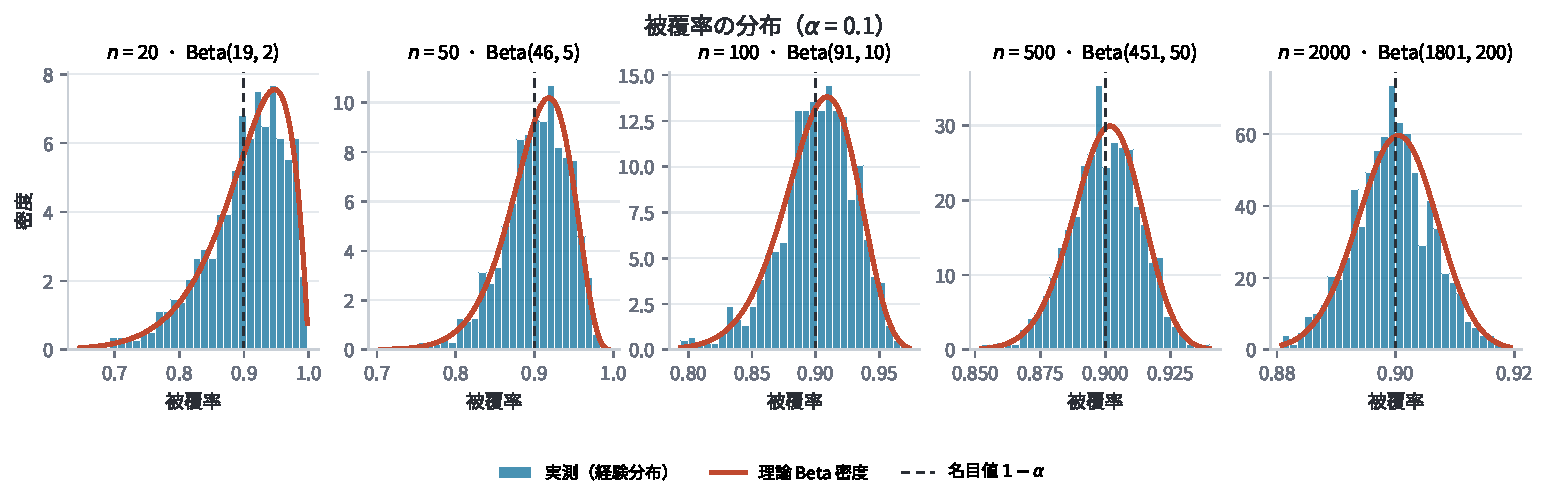
\includegraphics[width=\linewidth]{../figures/fig_e1_coverage_beta_alpha10.pdf}
  \caption{E1：被覆率の経験分布（ヒストグラム）と理論 $\mathrm{Beta}(k,\,n+1-k)$ の密度
    （$\alpha=0.10$、$R=1000$、テスト集合 $100{,}000$ 点）。破線は名目値 $1-\alpha$。
    $\alpha=0.05,\,0.20$ の図は \texttt{figures/fig\_e1\_coverage\_beta\_alpha05.pdf}、\texttt{alpha20.pdf}。}
  \label{fig:e1-beta}
\end{figure}

\begin{figure}[htbp]
  \centering
  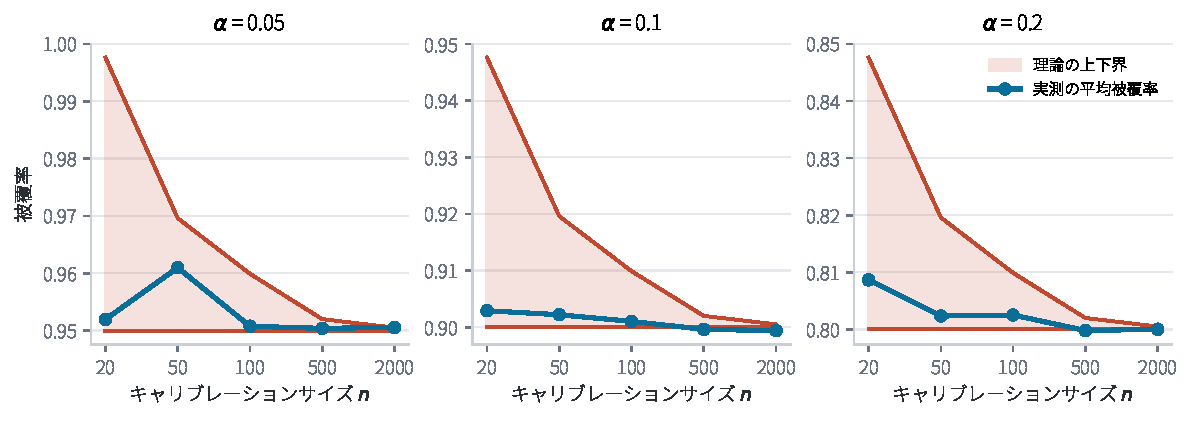
\includegraphics[width=\linewidth]{../figures/fig_e1_bounds.pdf}
  \caption{E1：平均被覆率（$R=1000$）と理論の上下界 $[\,1-\alpha,\ 1-\alpha+1/(n+1)\,]$。}
  \label{fig:e1-bounds}
\end{figure}

%% ===== 著者執筆（考察） =====
%% 論点：
%%  - n=2000 の 2 セルの KS 棄却の位置づけ：実装の誤りではなく、固定テスト集合による
%%    共通のずれ（0.14 SD）が R=1000 の KS で検出できる大きさだったこと。再評価で
%%    通ったことがその根拠（E1 仕様書「実行結果」「再評価」）
%%  - 「理論と合わない」ときに実装のバグか推定の分散かを切り分ける方法
%%    （テスト集合サイズを変える、in_bounds は鈍感、tests/ が通っているか。E1 仕様書「既知の注意点」）
%%  - 上下界の幅 1/(n+1) と試行ごとの被覆率のばらつき（Beta の SD）の関係。
%%    (n+1)α が整数のときの超過 0（命題 prop:excess。n=19, 99 は格子に無いので触れるなら注記）
%%  - 検証しているのは d を固定した段階の主張であること（d の引き直しは含まない）
%% 参照候補：\ref{thm:coverage}, \ref{cor:upper}, \ref{eq:two-sided}, \ref{prop:excess},
%%   \ref{thm:cond-coverage-beta}, \ref{cor:cond-coverage-moments}, \ref{rem:cond-coverage-assumptions},
%%   \ref{def:cond-coverage}, \ref{eq:coverage-rate}
%% =============================

\subsection{E1b：検証の水準と誤りの検出力}
\label{sec:e1b}
%% 仕様書: specs/E1b_detection_levels.md。実装: experiments/e1b_detection_levels.py。
%% 数値: results/e1b_detection_levels.csv。図: figures/fig_e1b_ecdf.pdf。

\paragraph{目的.}
被覆保証の検証には水準がある：L0 点推定を眺める、L1 下界 $1-\alpha$ を満たすか、
L2 上界 $1-\alpha+1/(n+1)$ も満たすか、L3 被覆率の分布が $\mathrm{Beta}(k,n+1-k)$ と
一致するか。どの水準がどの誤りを検出できるかを実演する。

\paragraph{手続き.}
$n=1000$、$\alpha=0.10$、$R=2000$ とし（$k=901$、理論分布 $\mathrm{Beta}(901,100)$、
平均 $0.90010$、標準偏差 $0.00947$、上下界 $[0.90000,\,0.90100]$）、次の $3$ ケースを
同じ較正集合で比べる。
\begin{enumerate}
  \item[(A)] \textbf{正しい実装}：$k=\lceil(n+1)(1-\alpha)\rceil$。
  \item[(B)] \textbf{誤実装}：$k=\lceil n(1-\alpha)\rceil$（$n+1$ を $n$ にする、最も典型的な誤り）。
  \item[(C)] \textbf{テスト集合が小さい}：実装は (A) と同じだが、被覆率を $2{,}000$ 点の
    テスト集合で推定する。
\end{enumerate}
(A)(B) の被覆率は $4{,}000{,}000$ 点のテスト集合で評価する（表~\ref{tab:exp-setup}）。

\paragraph{結果.}
表~\ref{tab:e1b-cases} に $3$ ケースの平均・標準偏差・理論との比較を示した。
図~\ref{fig:e1b-ecdf} は $3$ ケースの被覆率の経験分布関数と理論の分布関数である。
\begin{itemize}
  \item (A) は L1・L2・L3 のすべてを通る（平均 $0.90025$、$z=+0.72$、KS $p=0.911$）。
  \item (B) は平均 $0.89927$ で下界を下回り（L1 で検出）、$z=-3.94$、KS $p=1.28\times10^{-4}$
    （L3 でも検出）。(A) との平均の差は $0.001$ である。
  \item (C) は平均 $0.90038$ で L1・L2 を通る（$z=+1.33$）が、標準偏差が理論の $1.203$ 倍で、
    KS $p=1.53\times10^{-8}$（L3 でのみ検出）。
\end{itemize}
上下界の幅は $0.00100$、試行ごとの被覆率の標準偏差は $0.00947$ である。

\begin{figure}[htbp]
  \centering
  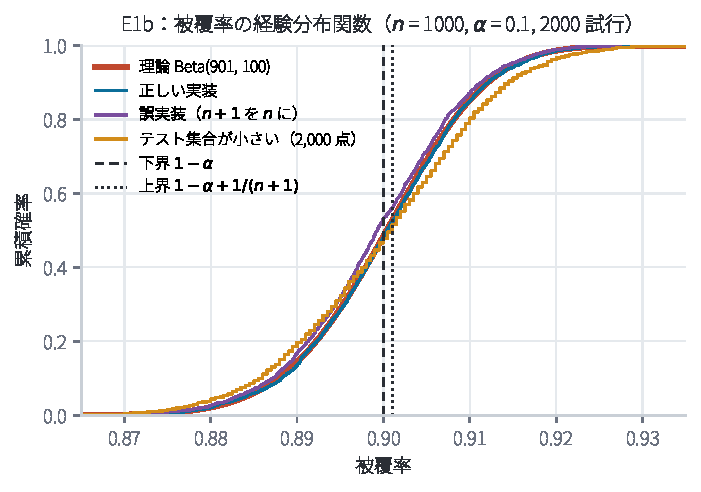
\includegraphics[width=0.8\linewidth]{../figures/fig_e1b_ecdf.pdf}
  \caption{E1b：$3$ ケースの被覆率の経験分布関数（階段）と理論 $\mathrm{Beta}(901,100)$ の
    分布関数（太線）。縦線は下界 $1-\alpha$ と上界 $1-\alpha+1/(n+1)$。
    出典：\texttt{results/e1b\_detection\_levels.csv}}
  \label{fig:e1b-ecdf}
\end{figure}

%% ===== 著者執筆（考察） =====
%% 論点：
%%  - 位置のずれは平均が、形のずれは分布が捕まえる。両方を見て初めて検証したと言える
%%  - off-by-one は被覆率を 0.001 しか動かさない（L0 では気づけない）が、位置のずれなので
%%    平均の検定でも分布の検定でも検出できる
%%  - 帯の幅 0.001 に対し試行ごとの SD 0.00947（約 10 倍）。1 回の実験では上下界を確かめられず、
%%    多数回の平均で初めて挟める
%%  - (C) の SD 比 1.203 と、加法性からの予測 1.225 の一致（5.1.2 の実例\encircle{2}に既述）
%%  - 平均を保ったまま分散だけを変える誤り（較正集合の使い回し、標本間の相関）を L3 が捕まえる。
%%    生成 AI が書いたコードを信用する根拠として L3 まで見ていること
%%  - 外部実装（MAPIE）との照合は本文に入れず、付録の検証の節で扱う
%%    （specs/E1b_detection_levels.md 末尾「付録に入れる候補」）
%% 参照候補：\ref{eq:khat}, \ref{rem:quantile-types}, \ref{thm:cond-coverage-beta}, \ref{prop:excess}
%% =============================

\subsection{E2：下敷きモデルへの非依存性}
\label{sec:e2}
%% 仕様書: specs/E2_model_agnostic.md。実装: experiments/e2_model_agnostic.py。
%% 数値: results/e2_summary.csv, e2_robustness.csv, e2_tiers.csv, e2_tier_pairs.csv。
%% 図: figures/fig_e2_model_agnostic.pdf, fig_e2_tier1_zoom.pdf。

\paragraph{目的.}
被覆率は下敷きモデルによらず一定であり、区間の幅だけがモデルの精度に応じて変わることを示す。

\paragraph{手続き.}
\eqref{eq:dgp-homo} の学習集合 $500$ 点を $1$ 回だけ生成し、\ref{sec:exp-setup}節の
$5$ モデルすべてを同じ学習集合で学習して固定する。テスト集合 $200{,}000$ 点の絶対残差を
モデルごとに計算しておく。$R=1000$ 回、較正集合 $500$ 点を引き直し（$5$ モデルで共有）、
各モデルの被覆率と幅 $2\qhat$ を記録する（$\alpha=0.10$、$k=451$、上下界
$[0.9000,\,0.9020]$）。主分析の後、学習集合と内部乱数を $5$ 通り（rep $0$〜$4$）に振り、
各 $200$ 試行で幅の順位が学習集合によらないかを確かめる。

\paragraph{結果.}
表~\ref{tab:e2-summary} と図~\ref{fig:e2-main} に主分析の結果を示す。
仕様書の判定基準 C1〜C4 の値は次のとおりである。
\begin{itemize}
  \item \textbf{C1（被覆はモデルによらない）}：$5$ モデルの平均被覆率はすべて上下界
    $[0.9000,\,0.9020]$ に入り、モデル間の最大差は $0.00091$ で、上下界の幅 $1/501=0.0020$
    より小さい。
  \item \textbf{C2（幅は精度に依存する）}：テスト集合の RMSE の順位と平均幅の順位の
    Spearman 順位相関は $1.0$。絶対残差の $0.90$ 分位点との順位相関も $1.0$。
  \item \textbf{C3（定数予測器でも被覆する）}：定数予測器の平均被覆率は $0.90046$ で
    $1-\alpha$ 以上。
  \item \textbf{C4（学習集合を超えて言えるか）}：$5$ 通りの学習集合で幅の順位は一致
    \textbf{しなかった}（表~\ref{tab:e2-robustness}）。定数予測器（常に $5$ 位）と
    リッジ回帰（常に $4$ 位）の順位は固定だが、勾配ブースティング・ニューラルネット・
    ランダムフォレストの $3$ つは $1$〜$3$ 位を入れ替わる。
\end{itemize}

\begin{table}[htbp]
  \centering
  \caption{E2 の主分析（学習集合 $1$ つに条件づけた結果、$R=1000$、$\alpha=0.10$、$n=500$）。
    被覆率の SE は試行間とテスト集合間（$N=200{,}000$）の $2$ 成分の合成
    \eqref{eq:se-composite}、幅の SE は試行間のみ。RMSE と $0.90$ 分位点は
    テスト集合での絶対残差のもの。出典：\texttt{results/e2\_summary.csv}}
  \label{tab:e2-summary}
  \small
  \begin{tabular}{lrrrrrr}
    \toprule
    モデル & 平均被覆率 & SE & 平均幅 & 幅の SE & RMSE & 残差の $0.90$ 分位点 \\
    \midrule
    定数予測器 & 0.90046 & 0.000798 & 2.9608 & 0.00308 & 0.9134 & 1.4762 \\
    リッジ回帰 & 0.90137 & 0.000789 & 2.2048 & 0.00260 & 0.6683 & 1.0961 \\
    ランダムフォレスト & 0.90046 & 0.000795 & 1.7869 & 0.00227 & 0.5410 & 0.8902 \\
    勾配ブースティング & 0.90070 & 0.000789 & 1.7736 & 0.00220 & 0.5375 & 0.8832 \\
    ニューラルネット & 0.90108 & 0.000788 & 1.8493 & 0.00235 & 0.5616 & 0.9198 \\
    \bottomrule
  \end{tabular}
\end{table}

\begin{table}[htbp]
  \centering
  \caption{E2 の頑健性確認：学習集合を $5$ 通りに振ったときの平均幅（各 $200$ 試行）と
    幅の順位（括弧内、$1$ が最も狭い）。出典：\texttt{results/e2\_robustness.csv}}
  \label{tab:e2-robustness}
  \small
  \begin{tabular}{lrrrrr}
    \toprule
    rep & 定数予測器 & リッジ回帰 & ランダムフォレスト & 勾配ブースティング & ニューラルネット \\
    \midrule
    0 & 2.9567（5） & 2.2086（4） & 1.7716（2） & 1.7606（1） & 1.8107（3） \\
    1 & 2.9566（5） & 2.2058（4） & 1.7841（3） & 1.7680（2） & 1.7305（1） \\
    2 & 2.9763（5） & 2.1989（4） & 1.7959（2） & 1.7965（3） & 1.7428（1） \\
    3 & 2.9684（5） & 2.2082（4） & 1.8165（2） & 1.8071（1） & 1.9144（3） \\
    4 & 2.9738（5） & 2.2106（4） & 1.8363（3） & 1.8129（2） & 1.7947（1） \\
    \bottomrule
  \end{tabular}
\end{table}

C4 が一致しなかったので、仕様書のとおり層構造として報告する（表~\ref{tab:e2-tiers}）。
モデルごとに rep 間の平均と標準偏差を求め、$10$ ペアすべてについて rep を対とする
対応あり $t$ 検定（自由度 $4$）を行い、Bonferroni 補正した有意水準 $0.05/10=0.005$ で
判定した。定数予測器・リッジ回帰を含む $7$ ペアは区別でき、勾配ブースティング・
ニューラルネット・ランダムフォレストの間の $3$ ペア（$p=0.040$、$0.94$、$0.77$）は
区別できない。したがって幅は $3$ つの層に分かれる：第 $1$ 層 \{勾配ブースティング、
ニューラルネット、ランダムフォレスト\}、第 $2$ 層 \{リッジ回帰\}、第 $3$ 層 \{定数予測器\}。
第 $1$ 層の拡大図を図~\ref{fig:e2-zoom} に示す。

\begin{table}[htbp]
  \centering
  \caption{E2 の層構造。rep 間（学習集合間）の平均幅・標準偏差、$t(4)$ による $95\,\%$ 区間、
    $5$ 通りの rep での順位の範囲。下段は対応あり $t$ 検定（自由度 $4$、Bonferroni 補正後の
    有意水準 $0.005$）。出典：\texttt{results/e2\_tiers.csv}, \texttt{results/e2\_tier\_pairs.csv}}
  \label{tab:e2-tiers}
  \small
  \begin{tabular}{llrrlc}
    \toprule
    層 & モデル & rep 間平均幅 & rep 間 SD & $95\,\%$ 区間 & 順位の範囲 \\
    \midrule
    1 & 勾配ブースティング & 1.7890 & 0.02347 & [1.7598, 1.8181] & 1--3 \\
    1 & ニューラルネット & 1.7986 & 0.07303 & [1.7079, 1.8893] & 1--3 \\
    1 & ランダムフォレスト & 1.8009 & 0.02583 & [1.7688, 1.8329] & 2--3 \\
    2 & リッジ回帰 & 2.2064 & 0.00454 & [2.2008, 2.2120] & 4--4 \\
    3 & 定数予測器 & 2.9664 & 0.00934 & [2.9548, 2.9780] & 5--5 \\
    \bottomrule
  \end{tabular}

  \medskip
  \begin{tabular}{lrrrc}
    \toprule
    ペア & 幅の差の平均 & $t$ & $p$ 値 & 区別できる \\
    \midrule
    定数予測器 -- リッジ回帰 & 0.7600 & 145.9 & 1.3e-08 & ○ \\
    定数予測器 -- ランダムフォレスト & 1.1655 & 129.2 & 2.2e-08 & ○ \\
    定数予測器 -- 勾配ブースティング & 1.1774 & 165.6 & 8e-09 & ○ \\
    定数予測器 -- ニューラルネット & 1.1678 & 35.8 & 3.6e-06 & ○ \\
    リッジ回帰 -- ランダムフォレスト & 0.4055 & 36.8 & 3.3e-06 & ○ \\
    リッジ回帰 -- 勾配ブースティング & 0.4174 & 39.5 & 2.5e-06 & ○ \\
    リッジ回帰 -- ニューラルネット & 0.4078 & 12.9 & 0.00021 & ○ \\
    ランダムフォレスト -- 勾配ブースティング & 0.0119 & 3.0 & 0.040 & × \\
    ランダムフォレスト -- ニューラルネット & 0.0023 & 0.1 & 0.945 & × \\
    勾配ブースティング -- ニューラルネット & -0.0096 & -0.3 & 0.766 & × \\
    \bottomrule
  \end{tabular}
\end{table}

\begin{figure}[htbp]
  \centering
  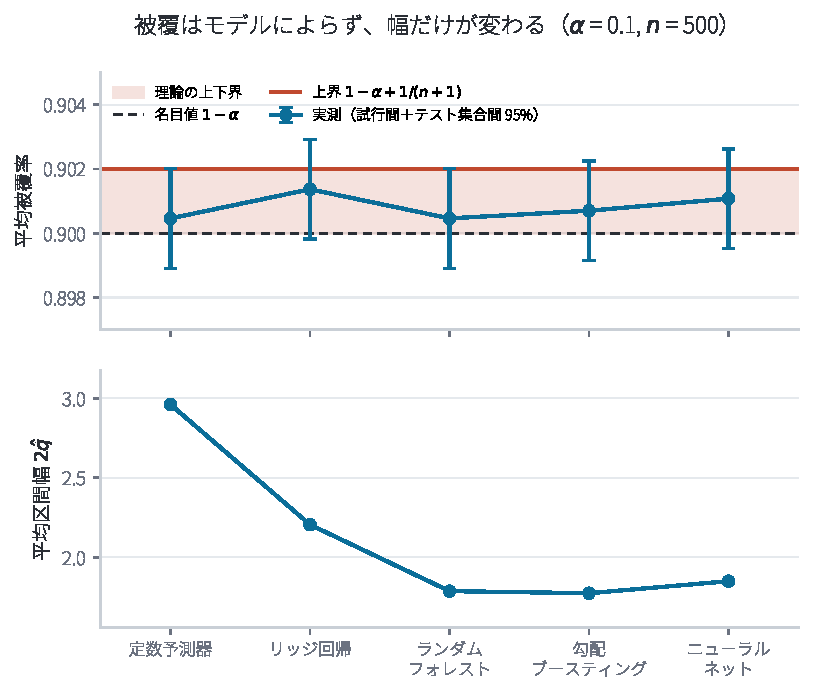
\includegraphics[width=0.85\linewidth]{../figures/fig_e2_model_agnostic.pdf}
  \caption{E2：$5$ つの下敷きモデルの平均被覆率（上段）と平均区間幅（下段）。
    上段の誤差棒は試行間とテスト集合間の $2$ 成分を合成した $95\,\%$ 区間、破線は名目値
    $1-\alpha$、実線は上界 $1-\alpha+1/(n+1)$。出典：\texttt{results/e2\_summary.csv},
    \texttt{results/e2\_robustness.csv}}
  \label{fig:e2-main}
\end{figure}

\begin{figure}[htbp]
  \centering
  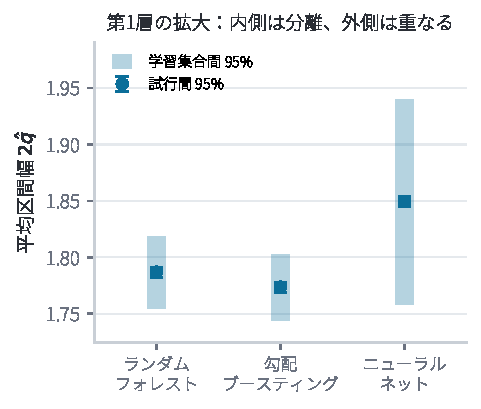
\includegraphics[width=0.7\linewidth]{../figures/fig_e2_tier1_zoom.pdf}
  \caption{E2：第 $1$ 層（勾配ブースティング・ニューラルネット・ランダムフォレスト）の
    平均幅の拡大図。誤差棒は rep 間（学習集合間）の $t(4)$ による $95\,\%$ 区間。
    出典：\texttt{results/e2\_tiers.csv}}
  \label{fig:e2-zoom}
\end{figure}

%% ===== 著者執筆（考察） =====
%% 論点：
%%  - 上段が平ら、下段が階段状。この対比自体が結論（被覆は不変、幅は変わる）
%%  - 保証は「正しさ」であって「有用性」ではない。定数予測器は被覆 0.90 を満たすが幅は使い物にならない
%%  - モデル選択は被覆の妥当性に影響せず、区間の情報量にのみ効く。予測モデルの改善努力は
%%    区間の妥当性ではなく狭さに効く
%%  - C2（試行間 SE で分離）と C4（学習集合間で分離）は別の問いに答えている。試行間 SE は
%%    「この学習集合のもとで」の主張にとどまる。これは周辺／条件付きの区別と同じ構造
%%    （5.1.2 の実例\encircle{3}に既述）
%%  - 層構造の報告は C4 が通るより情報量が多い（実験の分解能が分かる）
%%  - 定数予測器のテスト（tests/test_coverage_theory.py）はリーク検出の単体テスト、E2 は
%%    第5章に載せる実験結果。役割が違う
%% 参照候補：\ref{thm:coverage}, \ref{rem:assumptions}（A に条件を課さない）,
%%   \ref{rem:upper-meaning}（3：幅は保証しない）, \ref{prop:excess}（C1 の基準 1/(n+1)）, \ref{rem:marginal}
%% =============================

\subsection{E3：異分散データと条件付き被覆の破綻}
\label{sec:e3}
%% 仕様書: specs/E3_conditional_coverage.md。実装: experiments/e3_conditional.py、
%% experiments/e3_empty_interval_check.py（空区間の確認）。
%% 数値: results/e3_summary.csv, e3_marginal.csv, e3_empty_interval_check.csv。
%% 図: figures/fig_e3_band.pdf, fig_e3_stratified.pdf。

\paragraph{目的.}
周辺被覆が $1-\alpha$ を満たしていても、部分集団ごとの被覆は割れうる
（例~\ref{ex:x-conditional-hetero}）。不均一分散のデータ \eqref{eq:dgp-hetero} で、
(a) 絶対残差 \eqref{eq:score}、(b) 正規化残差 \eqref{eq:score-normalized}、
(c) CQR \eqref{eq:cqr-score} の周辺被覆と $X_1$ による層別被覆を測り、
(b)(c) が割れをどこまで縮めるかを比べる。

\paragraph{手続き.}
学習集合 $2{,}000$ 点で \ref{sec:exp-setup}節の下敷きモデル（(a)(b) は同じ $\fhat$、
(b) の $\hat\sigma$、(c) の $2$ 本の分位点回帰）を学習し、固定する。テスト集合
$200{,}000$ 点を全試行で共有し、$X_1$ の固定境界 $0.2/0.4/0.6/0.8$ で $5$ 層に分ける
（各層約 $40{,}000$ 点）。$R=500$ 回、較正集合 $1{,}000$ 点を引き直し（$3$ 手法で共有）、
各手法の $\qhat$、周辺被覆率、層別被覆率 \eqref{eq:stratified-coverage}、平均幅、
SSC \eqref{eq:ssc} を記録する（$\alpha=0.10$、$k=901$、上下界 $[0.90000,\,0.90100]$）。

\paragraph{結果：周辺被覆.}
表~\ref{tab:e3-marginal} に周辺量を示す。$3$ 手法の平均周辺被覆率は $0.90052$、
$0.90054$、$0.90122$ で、いずれも上下界に $\pm2\,\mathrm{SE}$ の許容で入る（C1）。
平均幅は絶対残差 $2.310$、正規化残差 $2.122$、CQR $2.038$ である。

\paragraph{結果：層別被覆.}
表~\ref{tab:e3-stratified} と図~\ref{fig:e3-stratified} に層別被覆率と層別の平均幅を示す。
\begin{itemize}
  \item \textbf{C2}：絶対残差の層別被覆は $0.9991/0.9903/0.9378/0.8413/0.7335$ と割れ、
    最大と最小の差（gap）は $0.2656$、最悪層（$X_1\in[0.8,1)$）の被覆率は $0.7335$ である。
  \item \textbf{C3}：gap は正規化残差 $0.0449$（絶対残差の $17\,\%$）、CQR $0.0740$（同 $28\,\%$）
    で、いずれも絶対残差の $1/2$ 以下。最悪層の被覆率は正規化残差 $0.8833$、CQR $0.8691$ で、
    いずれも絶対残差より $1-\alpha$ に近い。どちらも平らにはならない。
  \item \textbf{C4}：CQR の層別平均幅は $0.972/1.466/2.099/2.549/3.104$ と層番号とともに
    単調に増え（Spearman 順位相関 $1.0$）、最上位層と最下位層の幅の比は $3.19$
    （層の代表値での $\sigma$ の比は $5.0$）。正規化残差の比は $3.96$。絶対残差の幅は
    全層で $2.310$（比 $1.0$）。
\end{itemize}
図~\ref{fig:e3-band} は trial $0$ の絶対残差と CQR の区間の形である。

\paragraph{報告義務の $3$ 項目.}
CQR の分位点の交差率はテスト集合で $0.0$（交差した点なし）、$\hat\sigma$ の下限クリップの
発動率は $5\times10^{-5}$（テスト集合 $200{,}000$ 点中約 $10$ 点）、SSC の最悪層の被覆率は
正規化残差 $0.8847$、CQR $0.8840$、絶対残差は幅が定数のため層が $1$ つに潰れる
（表では「---」）。

\paragraph{空区間.}
CQR の $\qhat$ は $500$ 試行中 $2$ 試行で負（最小 $-0.00554$）であった。
注意~\ref{rem:cqr-negative} の 2 により $\qhat<0$ では
$\qhat_{\mathrm{hi}}(x)-\qhat_{\mathrm{lo}}(x)<-2\qhat$ となる $x$ で区間が空になりうるが、
テスト集合 $200{,}000$ 点での $\min_x(\qhat_{\mathrm{hi}}(x)-\qhat_{\mathrm{lo}}(x))=0.1010$
は $2|\min\qhat|=0.0111$ を上回り、空になった区間はない。

\begin{table}[htbp]
  \centering
  \caption{E3 の周辺量（$R=500$、$\alpha=0.10$、$n=1000$、上下界 $[0.90000,\,0.90100]$）。
    SE は試行間とテスト集合間（$N=200{,}000$）の $2$ 成分の合成 \eqref{eq:se-composite}。
    $\qhat$ と SSC 最悪層は試行平均。出典：\texttt{results/e3\_marginal.csv}}
  \label{tab:e3-marginal}
  \begin{tabular}{lrrrrr}
    \toprule
    手法 & 平均被覆率 & SE & 平均幅 & $\qhat$ & SSC 最悪層 \\
    \midrule
    絶対残差 & 0.90052 & 0.000806 & 2.3103 & 1.1552 & — \\
    正規化残差 & 0.90054 & 0.000785 & 2.1221 & 2.1502 & 0.8847 \\
    CQR & 0.90122 & 0.000793 & 2.0381 & 0.0643 & 0.8840 \\
    \bottomrule
  \end{tabular}
\end{table}

\begin{table}[htbp]
  \centering
  \caption{E3 の層別被覆率（上段。括弧内は試行間とテスト集合間を合成した $1.96\,\mathrm{SE}$、
    層内は各約 $40{,}000$ 点）と層別の平均幅（下段）。層は $X_1$ の固定境界 $0.2/0.4/0.6/0.8$。
    出典：\texttt{results/e3\_summary.csv}}
  \label{tab:e3-stratified}
  \footnotesize
  \setlength{\tabcolsep}{2.2pt}
  \begin{tabular}{lrrrrrrr}
    \toprule
    手法 & 層 1 & 層 2 & 層 3 & 層 4 & 層 5 & gap & 最悪層 \\
    \midrule
    絶対残差 & 0.9991 (0.0003) & 0.9903 (0.0010) & 0.9378 (0.0025) & 0.8413 (0.0039) & 0.7335 (0.0047) & 0.2656 & 0.7335 \\
    正規化残差 & 0.9283 (0.0026) & 0.8833 (0.0033) & 0.9078 (0.0029) & 0.8970 (0.0031) & 0.8864 (0.0032) & 0.0449 & 0.8833 \\
    CQR & 0.9431 (0.0026) & 0.9066 (0.0030) & 0.9091 (0.0029) & 0.8784 (0.0033) & 0.8691 (0.0034) & 0.0740 & 0.8691 \\
    \bottomrule
  \end{tabular}

  \medskip
  \begin{tabular}{lrrrrrrr}
    \toprule
    手法 & 層 1 & 層 2 & 層 3 & 層 4 & 層 5 & 幅の比（層 5/層 1） & Spearman \\
    \midrule
    絶対残差 & 2.3103 & 2.3103 & 2.3103 & 2.3103 & 2.3103 & 1.0000 & — \\
    正規化残差 & 0.8816 & 1.3616 & 2.1405 & 2.7365 & 3.4916 & 3.9607 & 1.0 \\
    CQR & 0.9719 & 1.4659 & 2.0990 & 2.5492 & 3.1044 & 3.1940 & 1.0 \\
    \bottomrule
  \end{tabular}
\end{table}

\begin{figure}[htbp]
  \centering
  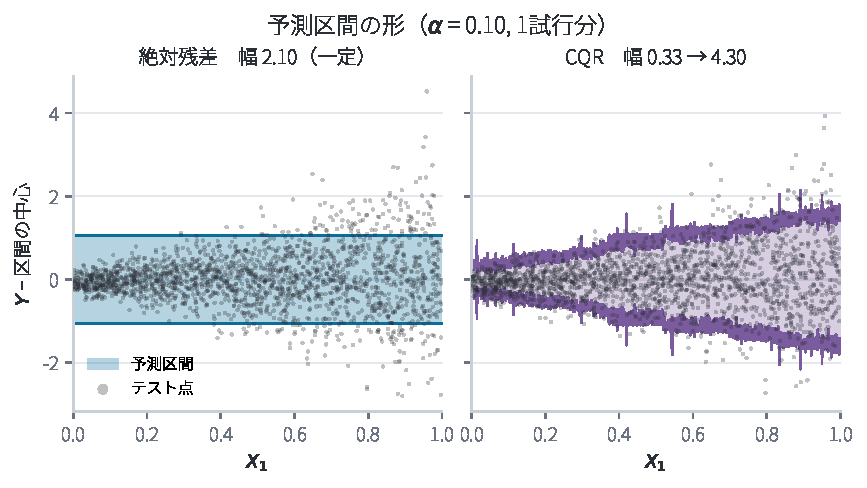
\includegraphics[width=\linewidth]{../figures/fig_e3_band.pdf}
  \caption{E3：trial $0$ の予測区間の形（左：絶対残差、右：CQR）。横軸は $X_1$、縦軸は
    $Y$ から区間の中心を引いた値（中心は $X_2$ にも依存するため、そのままでは帯にならない）。
    点は $2{,}000$ 点の無作為抽出。点が帯の内側にあることと $Y\in C(X)$ は同値なので、
    はみ出す点の割合がそのまま非被覆率である。出典：\texttt{results/e3\_band\_trial0.csv}}
  \label{fig:e3-band}
\end{figure}

\begin{figure}[htbp]
  \centering
  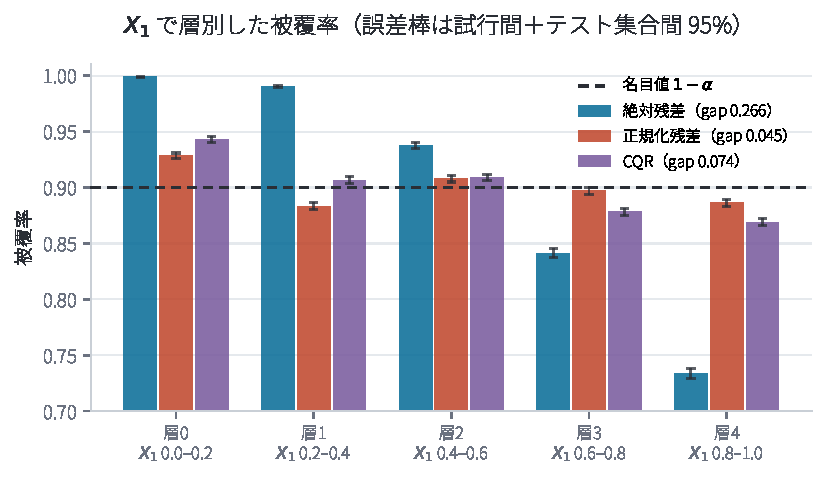
\includegraphics[width=0.85\linewidth]{../figures/fig_e3_stratified.pdf}
  \caption{E3：$X_1$ で層別した被覆率（$3$ 手法 $\times$ $5$ 層）。破線は名目値 $1-\alpha$。
    誤差棒は試行間とテスト集合間の $2$ 成分を合成した $95\,\%$ 区間。
    出典：\texttt{results/e3\_summary.csv}}
  \label{fig:e3-stratified}
\end{figure}

%% ===== 著者執筆（考察） =====
%% 論点：
%%  - 周辺被覆という保証は守られている。破綻しているのは「どの集団でも同じ精度で当たってほしい」
%%    という期待の方
%%  - 例 3.24（ex:x-conditional-hetero）との対応：n=1000, α=0.10 で k=901、周辺被覆の理論値
%%    901/1001 ≈ 0.90010、1−α との差 1/10010。絶対残差の最悪層 0.7335 の落ち込みはこれより
%%    桁違いに大きい
%%  - 層別が平らにならない理由の取り違え：不可能性定理が禁じるのは各点 x での条件付け。
%%    (a)(b)(c) が平らにならないのは単一の共形分位点で周辺較正しているから（(b)(c) の正規化が
%%    不完全なぶん残る）。層ごとの較正なら層別被覆は保証できる（prop:x-conditional-group）。
%%    E3 の層別被覆は診断量
%%  - (a) と (b) が同じ f̂ を共有するので、差は σ̂ の有無だけに帰属する。モデルの優劣ではなく
%%    スコアの設計が条件付き妥当性を左右する
%%  - 手法の順位：周辺的な効率（幅）では CQR、条件付きの妥当性（gap・最悪層）では正規化残差。
%%    理由：本 DGP は位置尺度族で正規化残差の特定が正しい（E|ε| の定数は q̂ が吸収）、
%%    分位点の推定は平均の推定より非効率で裾が不安定
%%  - 「CQR より正規化残差が優れている」と一般化してはならない。非対称誤差や位置尺度族から
%%    外れる設定では順序が入れ替わると予想（限界として明記するか E3b で確かめる。
%%    rem:normalized-limits の 2 が動機）
%%  - 固定ビンは実データでは使えない（第6章・今後の課題）
%%  - SSC が絶対残差で潰れるのは欠陥ではない
%%  - 交差率 0、クリップ 5e-5、空区間なしの位置づけ（後処理は保証に影響しない：rem:general-score の 2）
%% 参照候補：\ref{ex:x-conditional-hetero}, \ref{thm:x-conditional-impossible},
%%   \ref{prop:x-conditional-group}, \ref{rem:x-conditional-ch4}, \ref{def:x-conditional},
%%   \ref{prop:general-score}, \ref{rem:general-score}, \ref{rem:normalized-reduction},
%%   \ref{rem:normalized-limits}, \ref{rem:cqr-crossing}, \ref{rem:cqr-oracle}, \ref{rem:cqr-negative}
%% =============================

\subsection{E4：交換可能性が破れる場合}
%% TODO: 共変量シフト下で被覆が名目値を下回ること。重み付きによる部分的回復。

\subsection{E5：学習／較正の分割比}

\subsection{E6：jackknife+・CV+ とのデータ効率比較}

\subsection{考察}

%%=====================================================================
\section{実データ解析}
%%=====================================================================

\subsection{データ}
%% TODO: UCI Machine Learning Repository から2〜3件。入手手順は別途提出。

\subsection{結果}

\subsection{考察}

%%=====================================================================
\section{結論と今後の課題}
%%=====================================================================

\subsection{本論文で明らかにしたこと}
%% TODO: 3つのRQへの回答。
%%   保証は理論の上下界どおりに成り立ち、被覆率の分布まで理論と一致する。
%%   一方その保証は周辺被覆に限られ、区間の有用性も条件付き妥当性も保証の外にある。

\subsection{本研究の限界}

\subsection{今後の課題}
%% TODO: 条件付き被覆の近似的改善（Mondrian等）、時系列への拡張（ACI, EnbPI）、
%%       分類への適用。

%%=====================================================================
\appendix
%%=====================================================================

\section{数式と実装の対応表}
%% TODO: 本文の式番号と、src/ の関数名を対応させた表。
%%       ★これは必ず入れること。実装を理解している証拠になり、口頭試問でも効く。

\section{実験環境と再現手順}
%% TODO: Python 3.11 / numpy, scipy, scikit-learn, pandas, matplotlib
%%       乱数シード、実行コマンド、所要時間。

\section{生成AIの利用について}
%% TODO: docs/AI利用の記載.md の文案をそのまま入れる。
%%       利用範囲・利用しなかった範囲・検証体制の3点を書く。

%%=====================================================================
%% \nocite{*} は refs.bib の全件を強制的に引用扱いにして、本文の \cite が
%% まだ無い段階でも参考文献リストを生成させるためのもの。
%% **第2締切までに削除する（本文の \cite に置き換わったら不要）。**
%% 提出要件（docs/提出要件と締切.md 第4節）により pbibtex の Warning は残せないので、
%% 12件をまとめて今のうちに検証する目的で置いている。
\nocite{*}
\bibliographystyle{jplain}   %% 先生指定のスタイルに合わせること
\bibliography{refs}
%%=====================================================================

\end{document}
